\documentclass[a4paper,12pt]{report}

\usepackage{alltt, fancyvrb, url}
\usepackage{graphicx}
\usepackage[utf8]{inputenc}
\usepackage{float}
\usepackage{xcolor}
\usepackage{hyperref}

% Questo commentalo se vuoi scrivere in inglese.
\usepackage[italian]{babel}

\usepackage[italian]{cleveref}

\title{Relazione per\\``Programmazione ad Oggetti''}

\author{Simone Alocchi\\simone.alocchi@studio.unibo.it
\\Enrico Ancarani\\enrico.ancarani@studio.unibo.it
\\Stefano Baiano\\stefano.baiano@studio.unibo.it
\\Andrea Monti\\andrea.monti24@studio.unibo.it}
\date{\today}


\begin{document}

\maketitle

\tableofcontents

\chapter{Analisi}

\section{Descrizione e requisiti}

Il software ha come obiettivo di creare una copia del gioco da tavolo "Il Labirinto Magico" della Ravensburger.
%
L'intento principale è di riprodurre le dinamiche e le meccaniche del gioco
 originali, ma con l'aggiunta di elementi nuovi come per esempio i 
powerUps e un nemico che si muove all'interno del labirinto.
%
Il gioco si sviluppa su un'idea di competizione diretta tra i giocatori,
 configurandosi quindi come un'esperienza di tipo "tutti contro tutti".

\subsection*{Requisiti funzionali}
\begin{itemize}
	\item L’utente può avviare una partita scegliendo da 2 a 4 giocatori.
	%
	In base al numero di giocatori selezionati, varieranno le dimensioni del labirinto e la gestione dei turni.
	%
	Tutti i giocatori devono essere controllati manualmente, quindi si consiglia di giocare insieme ad amici.
	\item Il labirinto deve essere generato con una dimensione fissa che varia in base al numero di giocatori presenti.
	%
	Questa scelta riguarda esclusivamente la fase iniziale della partita: il labirinto potrà poi essere modificato durante il gioco.
	\item Il gioco permette di modificare il labirinto inserendo la tessera rimasta fuori dalla generazione iniziale.
	%
	Inserendo la tessera da uno dei lati del labirinto, tutte le tessere nella riga o colonna corrispondente si spostano di una posizione.
	%
	La tessera che esce dal lato opposto diventa la nuova tessera disponibile per la modifica al turno successivo.
	\item All'interno del labirinto vengono generati degli obiettivi che i giocatori possono raccogliere.
	\item Ogni volta che un giocatore raccoglie un obiettivo, riceve un power-up a utilizzo singolo.
	\item In ogni momento, l’interfaccia grafica mostra una classifica aggiornata con i nomi dei giocatori e i loro punteggi attuali.
	\item L'utente può decidere di giocare con all'interno del labirinto un nemico con movimento casuale.
	\item L’interfaccia grafica si aggiorna automaticamente dopo ogni azione compiuta.
\end{itemize}

\subsection*{Requisiti non funzionali}
\begin{itemize}
	\item Creare un nemico intelligente che se possibile insegue il giocatore.
	\item Salvataggio e caricamento di una partita giocata in precedenza e non finita.
\end{itemize}

\section{Modello del Dominio}

Il sistema rappresenta un gioco da tavolo digitale ambientato in un labirinto dinamico. Il labirinto viene generato con tessere posizionate casualmente. 
I giocatori partono dagli angoli della mappa, mentre un nemico viene inizialmente posizionato al centro. 
Gli obiettivi da raccogliere sono distribuiti in tessere casuali all'interno del labirinto.
Ogni volta che un turno inizia si eseguono 3 fasi in questa sequenza:
\begin{itemize}
	\item Fase di modifica: Il giocatore inserisce la tessera esterna in uno dei lati del labirinto ruotata a suo piacimento, facendo slittare la riga o la colonna corrispondente. Questo cambia dinamicamente la forma del labirinto.
	\item Fase del Giocatore: Il giocatore può:
	\begin{itemize}
		\item Muoversi all’interno del labirinto senza limiti di passi, in base alle connessioni disponibili tra le tessere.
		\item Usare un eventuale power-up ottenuto precedentemente.
	\end{itemize}
	\item Fase del Nemico: Il nemico si muove secondo una logica definita e se entra in contatto con un giocatore, gli rimuove un obiettivo raccolto e lo riposiziona nel labirinto.
\end{itemize}
Durante la partita, i giocatori devono cercare di raccogliere il maggior numero possibile di obiettivi. Ogni obiettivo raccolto fornisce al giocatore un power-up utilizzabile una sola volta.
Al termine del gioco (quando tutti gli obiettivi sono stati raccolti), vince il giocatore che ne ha ottenuti di più.
In caso di parità, viene generato un ulteriore obiettivo per determinare il vincitore continuando la partita.

\begin{figure}[H]
	\centering{}
	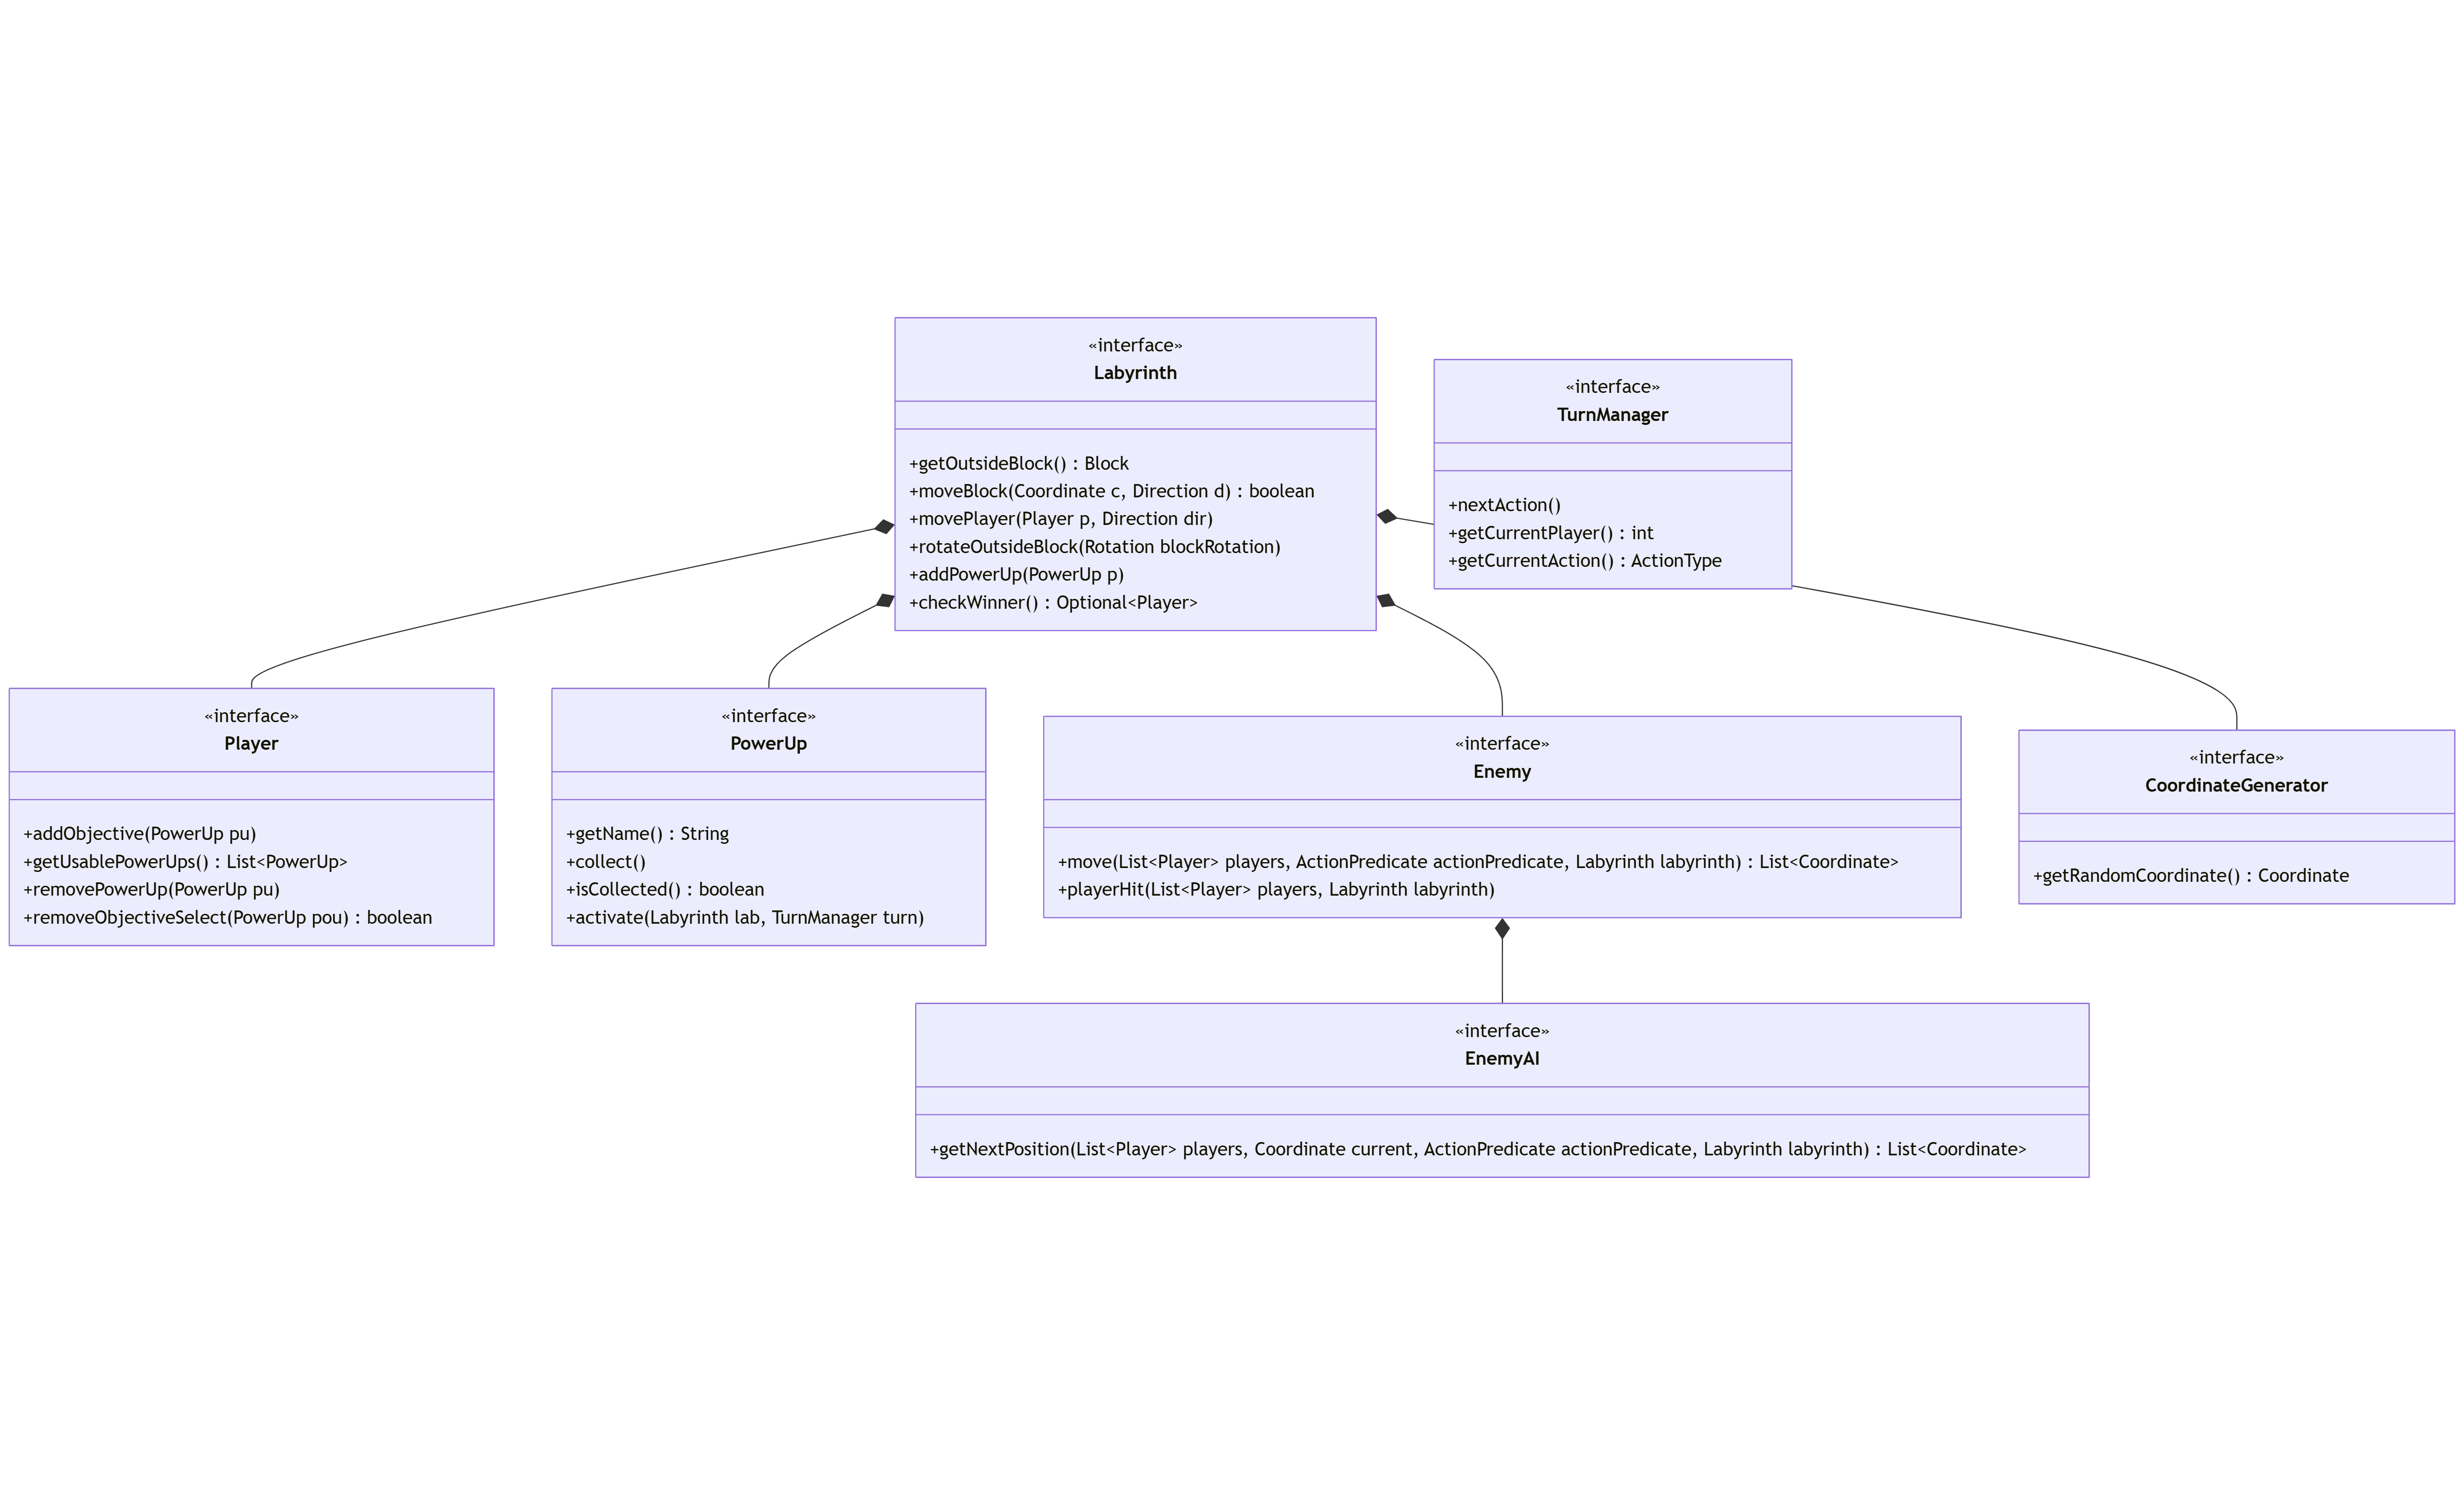
\includegraphics[width=14cm]{img/DominioElementi.png}
	\caption{Schema UML del dominio per la parte degli elementi}
	\label{img:dominio elementi}
\end{figure}

\begin{figure}[H]
	\centering{}
	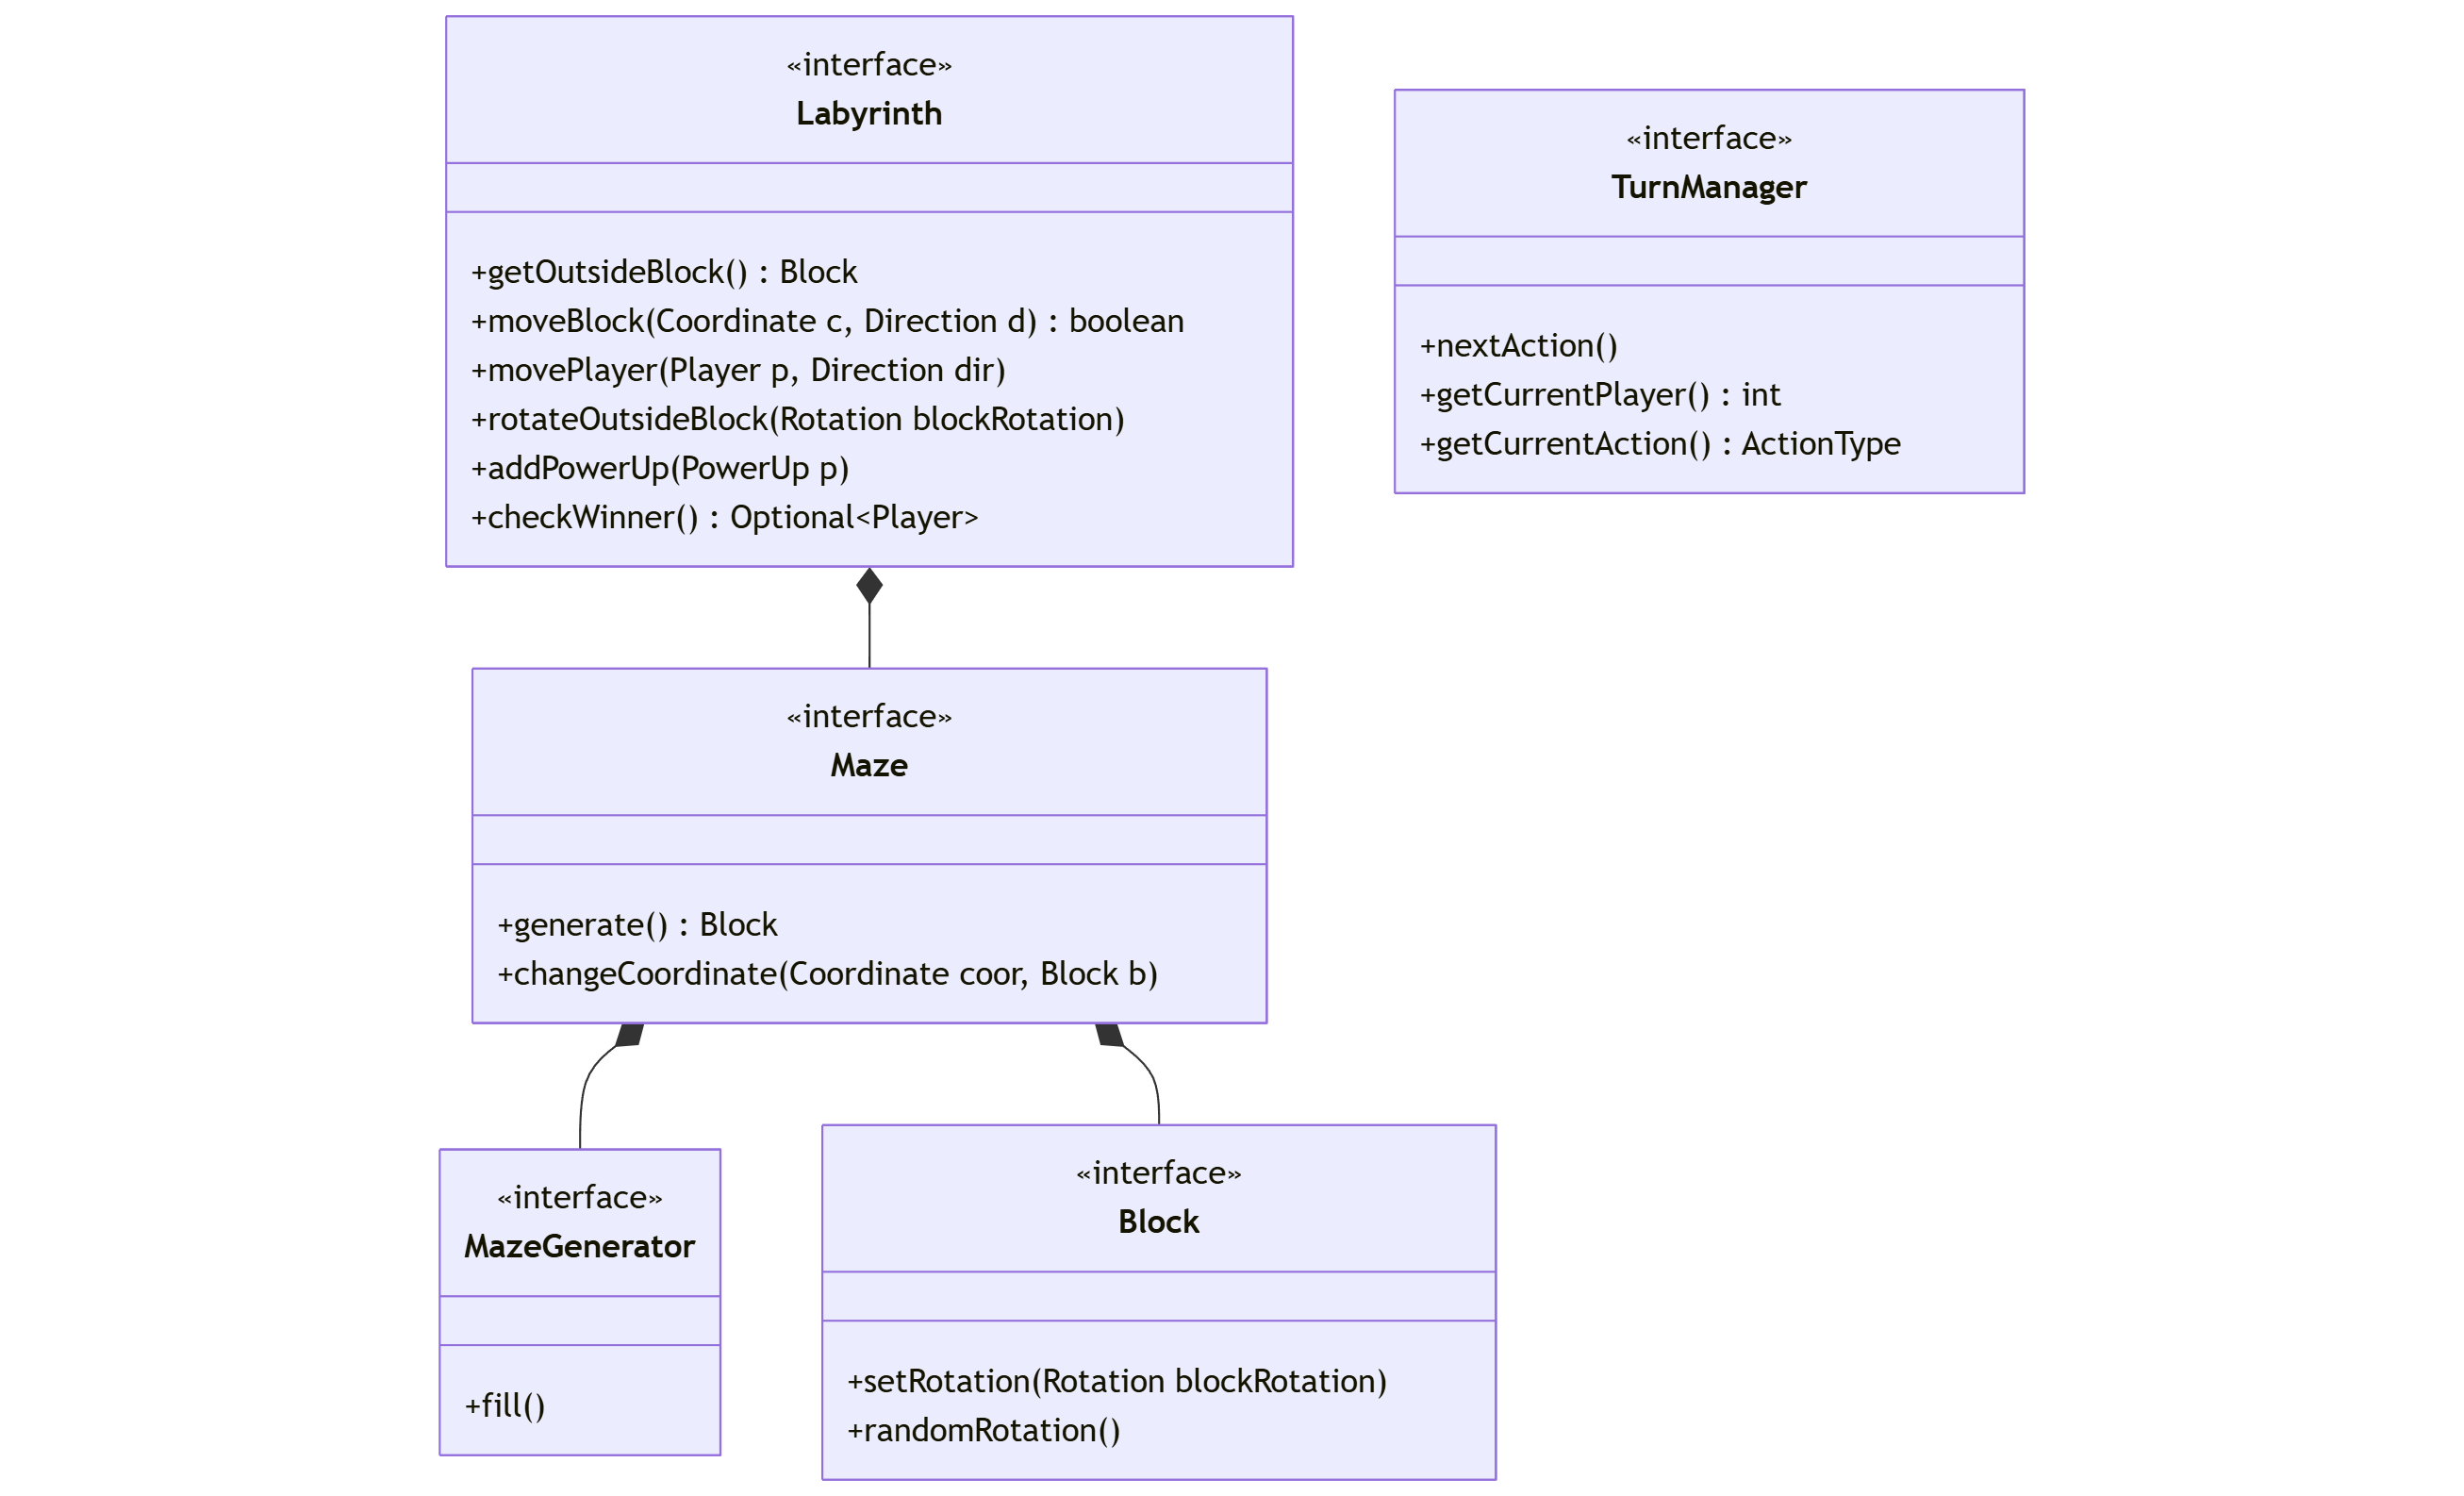
\includegraphics[width=14cm]{img/DominioLabirinto.png}
	\caption{Schema UML del dominio per la parte del labirinto}
	\label{img:dominio labirinto}
\end{figure}

\chapter{Design}

\section{Architettura}
Il progetto è strutturato secondo il pattern architetturale MVC (Model-View-Controller). 
Il punto di partenza dell’interazione fra utente e software inizia con la view MainMenu, la quale offre diverse opzioni:
\begin{itemize}
	\item Avviare una nuova partita.
	\item Caricare una partita salvata.
	\item Accedere alle impostazioni di gioco.
	\item Uscire dall’applicazione.
\end{itemize}
La parte logica del MainMenu viene affidata ad un MainMenuController, 
il quale compie operazioni con la view SettingsMenu ed il LoadController, che serviranno a gestire l’avvio della partita e il cambiamento delle impostazioni di gioco.
Se si seleziona di accedere alle impostazioni di gioco verrà mostrata la view SettingsMenu che permette all’utente di configurare i parametri di gioco, quali:
\begin{itemize}
	\item Difficoltà del nemico.
	\item Numero di giocatori.
	\item Numero di power-up/obiettivi disponibili.
	\item Se il nemico è presente.
\end{itemize}
Il settingsController, come nel caso del MainMenuController, si occupa delle operazioni logiche, 
quali il salvataggio delle impostazioni appena scelte dall’utente tramite la classe  SaveController, in grado di scrivere su file.
In caso di avviamento o di caricamento della partita precedente il MainMenuController richiamerà alcune funzioni del 
LoadController, che raccoglieranno a seconda del caso i dati dei settings oppure la partita precedente, attraverso i file di salvataggio.
All’avviamento della partita viene creato un GameController che genererà tutti gli elementi del gioco tramite una classe Builder, 
e li assegnerà alle classi sottostanti. Inoltre, il GameController si occuperà della coordinazione delle componenti principali quali:
\begin{itemize}
	\item Labyrinth, che rappresenta l’ambiente di gioco con tutti i suoi elementi.
	\item TurnManager, responsabile della gestione dei turni tra i giocatori.
	\item ActionController, gestore delle azioni e delle loro conseguenze.
	\item SaveController, per il salvataggio automatico dello stato di gioco.
\end{itemize}
A seguito viene creata la view principale del gioco, la GameView, responsabile dell’interfaccia tra utente ed il gioco. Questa si occupa di:
\begin{itemize}
	\item Creare gli elementi dell’interfaccia (pulsanti, label, ecc.).
	\item Aggiornare i componenti grafici in base ai cambiamenti nel model.
	\item Visualizzare lo stato corrente del gioco (punteggi, turno corrente, ecc.).
	\item Permettere l’interazione dell’utente con i suoi elementi.
\end{itemize}
Le operazioni logiche, anche in questo caso, sono delegate ad un’altra classe, la LogicGameView, che funge da intermediario tra GameView e GameController, 
offrendo metodi per ottenere informazioni sullo stato del gioco e per eseguire azioni in risposta agli input dell’utente.
Questi input utente vengono elaborati dall’ActionController, che determina il tipo di azione da eseguire e la applica al model. 
Prima di eseguire un’azione, consulta l’ActionPredicate, un componente di tipo ”semaforo” che stabilisce se un’azione è eseguibile 
in base alle condizioni attuali del model. Dopo ogni azione, la GameView si aggiorna.
\begin{figure}[H]
	\centering{}
	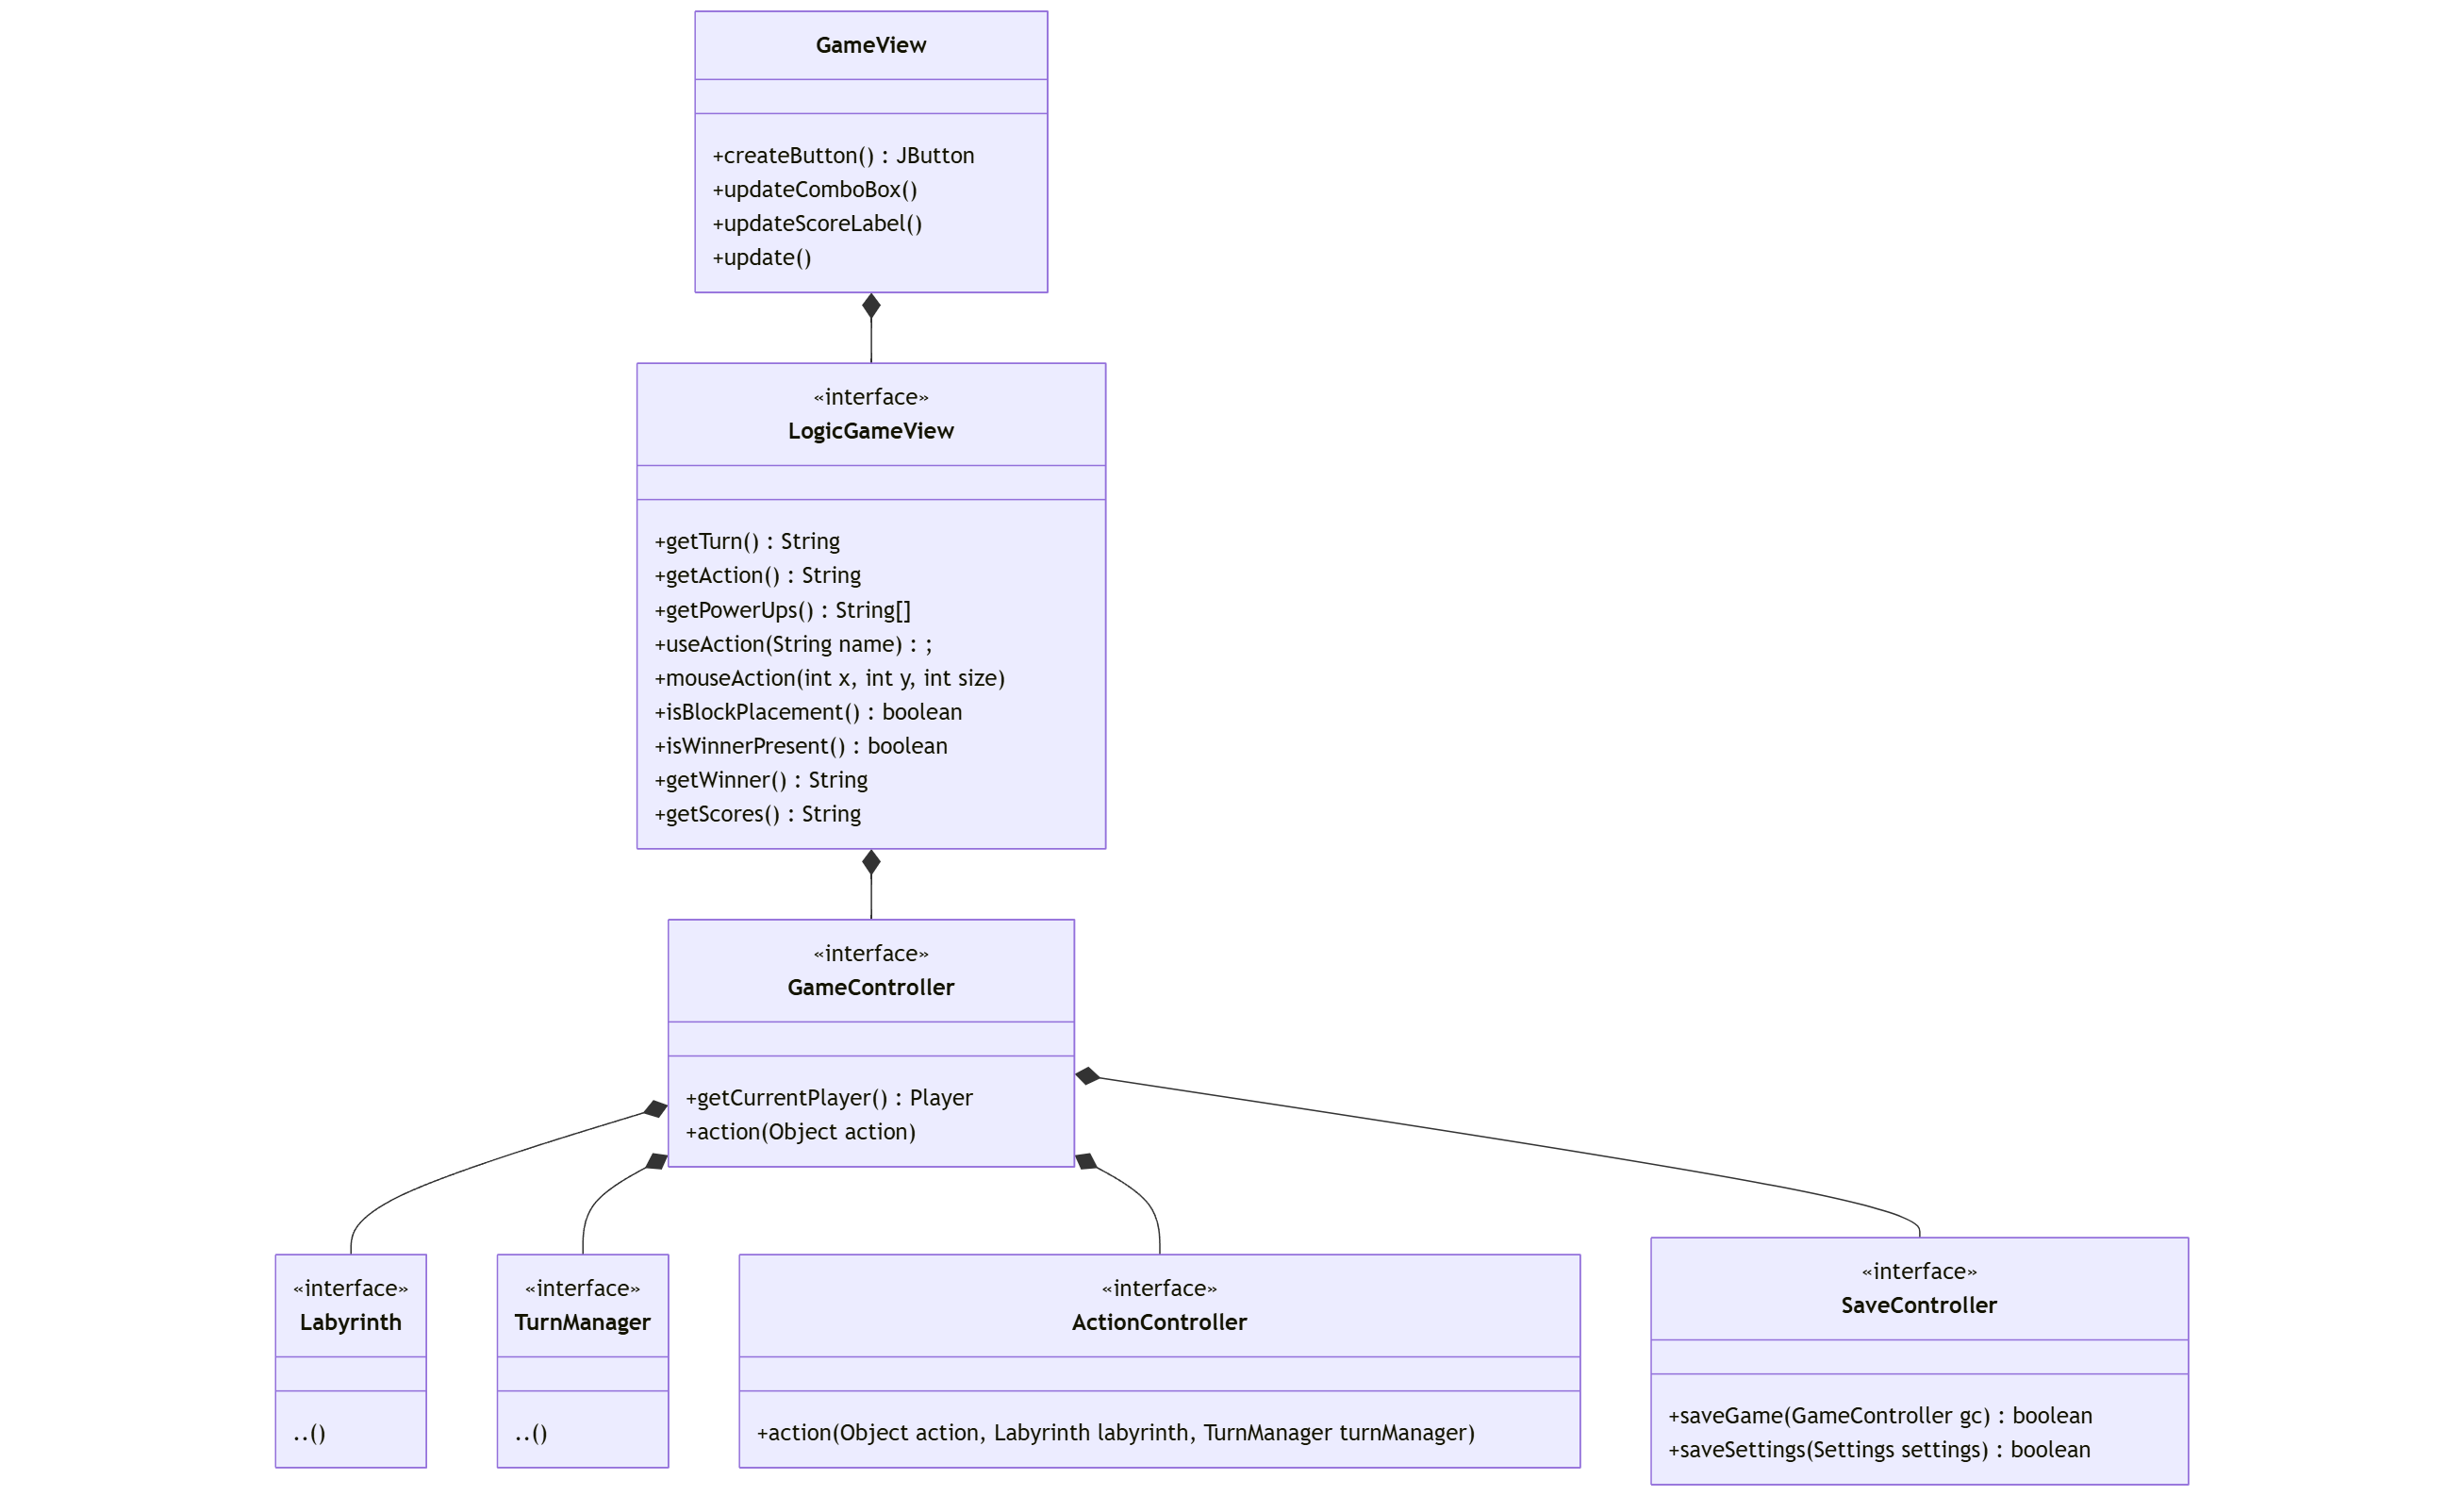
\includegraphics[width=14cm]{img/ArchitetturaGameView.png}
	\caption{Schema UML dell'architettura per la parte di gioco}
	\label{img:Architettura GameView}
\end{figure}

\section{Design dettagliato}

\subsection{Enrico Ancarani}
\textbf{Generazione del labirinto}
\\
\\
\textbf{PROBLEMA}\\
Nel gioco originale Labirinto Magico di Ravensburger, la composizione delle tessere è fissa: ci sono un numero predefinito di tessere a "L", a "T" e a linea retta, 
e la difficoltà e la giocabilità derivano dalla loro disposizione e rotazione. Tuttavia, il nostro gioco prevede la possibilità di cambiare le dimensioni del labirinto 
in base al numero di giocatori, rendendo impraticabile copiare esattamente il contenuto del gioco originale.
Inoltre, una generazione completamente casuale delle tessere rischia di rendere il labirinto poco giocabile: troppe tessere dello stesso tipo 
possono compromettere l’esperienza dell’utente.\\
\\
\textbf{SOLUZIONE}\\
Per risolvere questo problema, ho definito una gerarchia di classi orientata all’estensione e alla flessibilità.
\begin{itemize}
	\item \textbf{Maze}: è una classe astratta che definisce l’interfaccia e le funzionalità comuni di qualsiasi tipo di labirinto.
	\item \textbf{SimpleMaze}: è un’implementazione di Maze che utilizza la stessa composizione di tessere del gioco originale.
	\item \textbf{MazeGenerator}: è la classe responsabile della costruzione del labirinto: riceve in input un insieme predefinito di tessere 
	(fornite dalla sottoclasse di Maze), le posiziona sulla griglia assegnando a ognuna una coordinata e impendendo alla tessera di 
	essere riposizionata, e restituisce il labirinto completato con una tessera “extra” da usare per la meccanica di shift.
\end{itemize}
Durante la progettazione ho stabilito che le quattro posizioni di spawn dei giocatori (i quattro angoli del labirinto) 
devono contenere sempre tessere a “L” ruotate verso il centro, per garantire un inizio bilanciato e impedire generazioni scomode per i giocatori all'inizio. (labirinto di tessere angolo)
\\
\\
\textbf{PRO}
\begin{itemize}
	\item Facile estensione per diversi tipi di labirinti: Si possono creare estensioni di Maze che permettono in futuro all'utente di scegliere mappe di gioco con conformazioni 
	particolari.
	\item Chiarezza nella separazione di responsabilità: La gestione delle coordinate delle tessere viene fatta dal Maze, la generazione e assegnazione iniziale dal MazeGenerator e 
	la scelta di tessere dal SimpleMaze
	\item Template Method Pattern: viene utilizzato questo pattern per creare un ambiente facilmente estensibile e lasciare il comportamento generale del labirinto invariato.
\end{itemize}
\textbf{CONTRO}
\begin{itemize}
	\item È necessario implementare una nuova sottoclasse per ogni tipo di configurazione: ogni volta che si vuole un certo scenario con una scelta specifica di tessere bisogna 
	implementare una nuova sottoclasse di Maze
\end{itemize}
\begin{figure}[H]
	\centering{}
	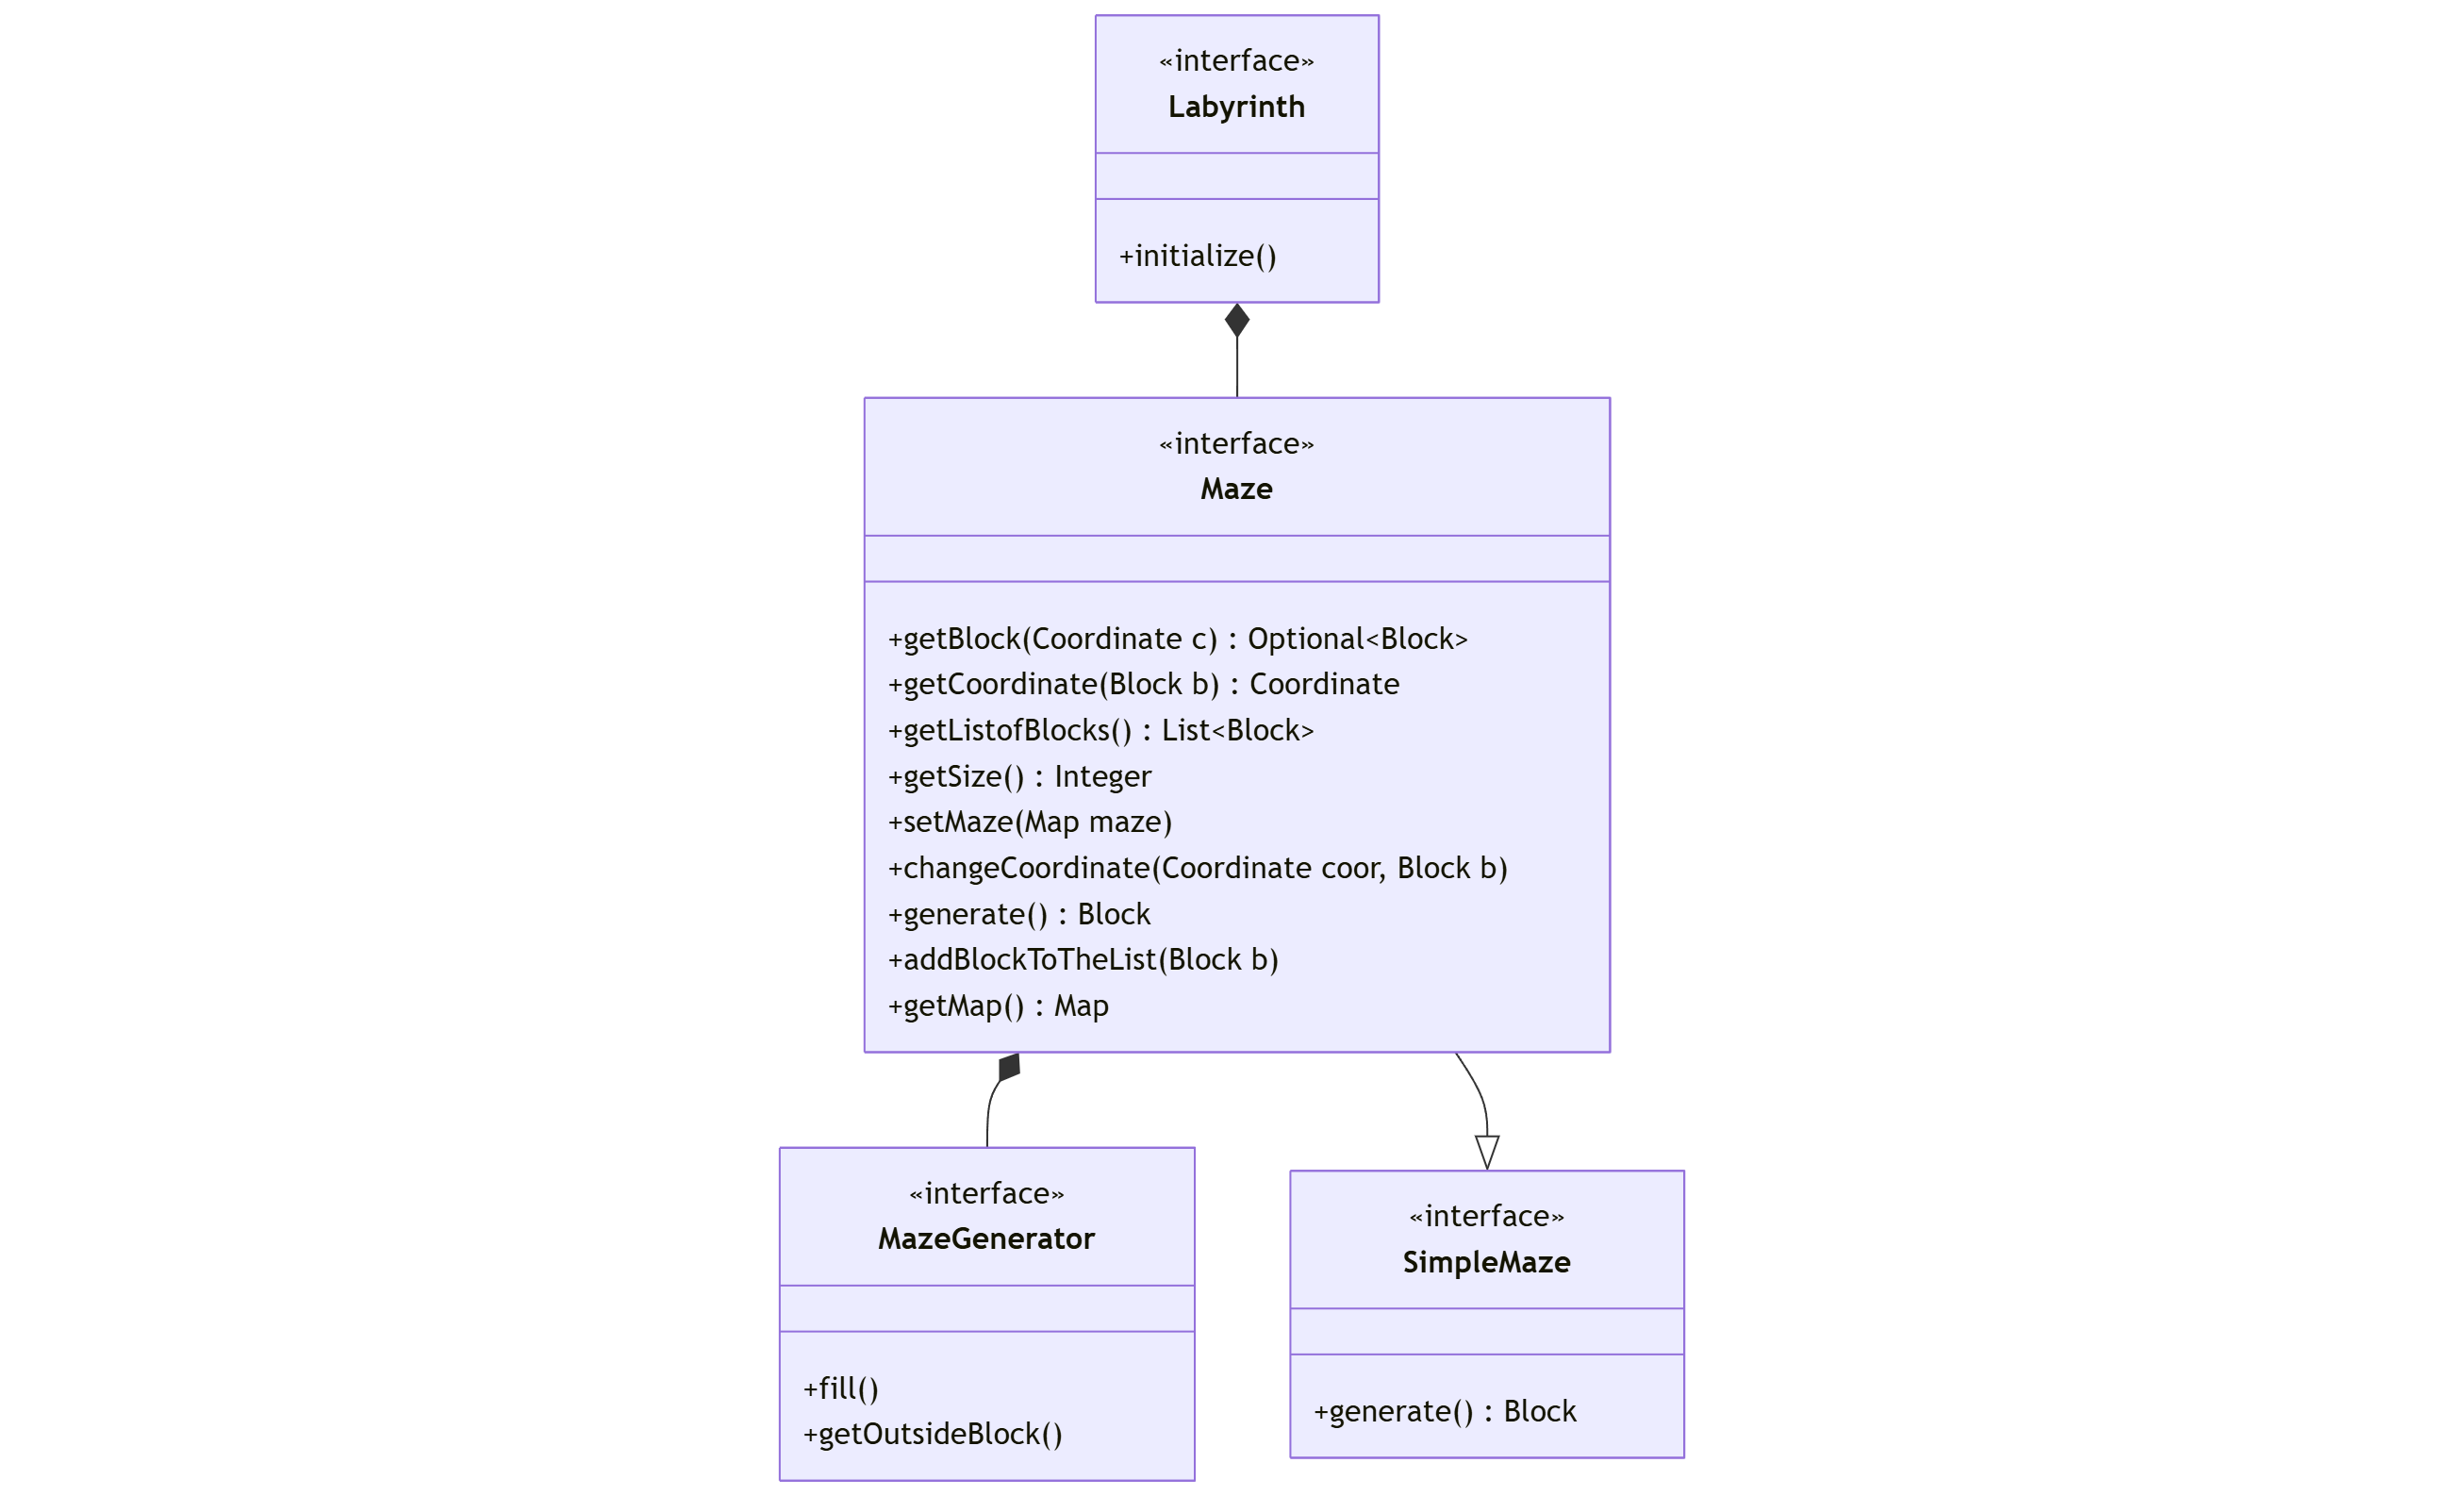
\includegraphics[width=14cm]{img/GenerazioneLabirinto.png}
	\caption{Schema UML della struttura per generare il labirinto}
	\label{img:Generazione Labirinto}
\end{figure}
\textbf{Gestione delle coordinate e coordinate iniziali}
\\
\\
\textbf{PROBLEMA}\\
Un aspetto centrale nello sviluppo del gioco è la gestione delle posizioni degli elementi sulla mappa.
Essa viene con diverse problematiche da risolvere:
\begin{itemize}
	\item Recupero della posizione: necessità di ottenere le coordinate a partire da un elemento e viceversa.
	\item Meccanica di shift: gestione dello spostamento delle tessere (e degli elementi sopra di esse) a seguito dell’inserimento della tessera extra.
	\item Effetto "Pac-Man": se un elemento viene spinto fuori dal labirinto, deve riapparire dalla parte opposta, mantenendo coerenza con la direzione dello spostamento.
\end{itemize}
\textbf{SOLUZIONE}\\
Una possibile soluzione iniziale era lasciare che ogni elemento conoscesse 
la propria posizione, ma questa scelta avrebbe complicato eccessivamente 
l’interazione tra elementi e labirinto. Pertanto, ho optato per un approccio centralizzato.
Per risolvere le problematiche sopra descritte, ho progettato la classe Labyrinth, 
responsabile della gestione centralizzata delle coordinate di tutti gli elementi del gioco: giocatori, nemico e powerup (obbiettivi).
Al suo interno la classe utilizza 2 componenti creati appositamente:
\begin{itemize}
	\item \textbf{DualMap}: struttura bidirezionale che collega elementi e coordinate, permettendo sia di trovare la posizione di un elemento, 
	sia di identificare cosa si trova in una determinata posizione.
	\item \textbf{CoordinateGenerator}: classe dedicata alla generazione delle coordinate iniziali, secondo logiche diverse in base al tipo di elemento.
\end{itemize}
La classe CoordinateGenerator è progettata per supportare la generazione delle coordinate in base alle seguenti esigenze:
\begin{itemize}
	\item PowerUp: la generazione avviene escludendo gli angoli del labirinto (riservati ai giocatori).
	\item Nemico: viene determinata la coordinata centrale del labirinto (calcolata sulla base della dimensione).
	\item Giocatori: la generazione avviene estraendo randomicamente i 4 angoli della mappa.
\end{itemize}
In ogni caso, le coordinate già estratte vengono rimosse dal set interno, garantendo unicità e prevenendo sovrapposizioni indesiderate.
Per quanto riguarda la meccanica di shift ho pensato che potesse bastare un metodo all'interno della classe Labyrinth.
Ho pensato che la responsabilità del metodo ricadesse proprio nel Labyrinth in quanto il metodo shift è alla base uno spostamento di coordinate.
Per funzionare al meglio ho deciso di suddividere i compiti del metodo su più metodi private in modo da permettere una chiara lettura e modifica.
Le funzioni suddivise sono: Determinare il tipo di shift (riga,colonna), calcolare la nuova posizione per ogni elemento, modificare la posizione delle tessere, modificare la posizione degli elementi,
controllare se la nuova posizione è fuori dal labirinto e se lo è modificarla.
\\
\\
\textbf{PRO}
\begin{itemize}
	\item Centralizzazione della gestione delle coordinate, riducendo al minimo il numero di chiamate e sincronizzazioni necessarie tra elementi e mappa.
	\item Facilità di estensione: la suddivisione delle responsabilità consente di introdurre nuove politiche di posizionamento (es. nuove entità) con impatto minimo sul codice esistente.
	\item Separazione delle responsabilità ben definita, che migliora leggibilità e manutenibilità del codice.
\end{itemize}
\textbf{CONTRO}
\begin{itemize}
	\item Gli elementi che necessitano di accedere alle posizioni di altri oggetti (ad esempio per calcoli di targeting) devono ricevere un 
	riferimento al Labyrinth o alla rispettiva DualMap.
\end{itemize}
\begin{figure}[H]
	\centering{}
	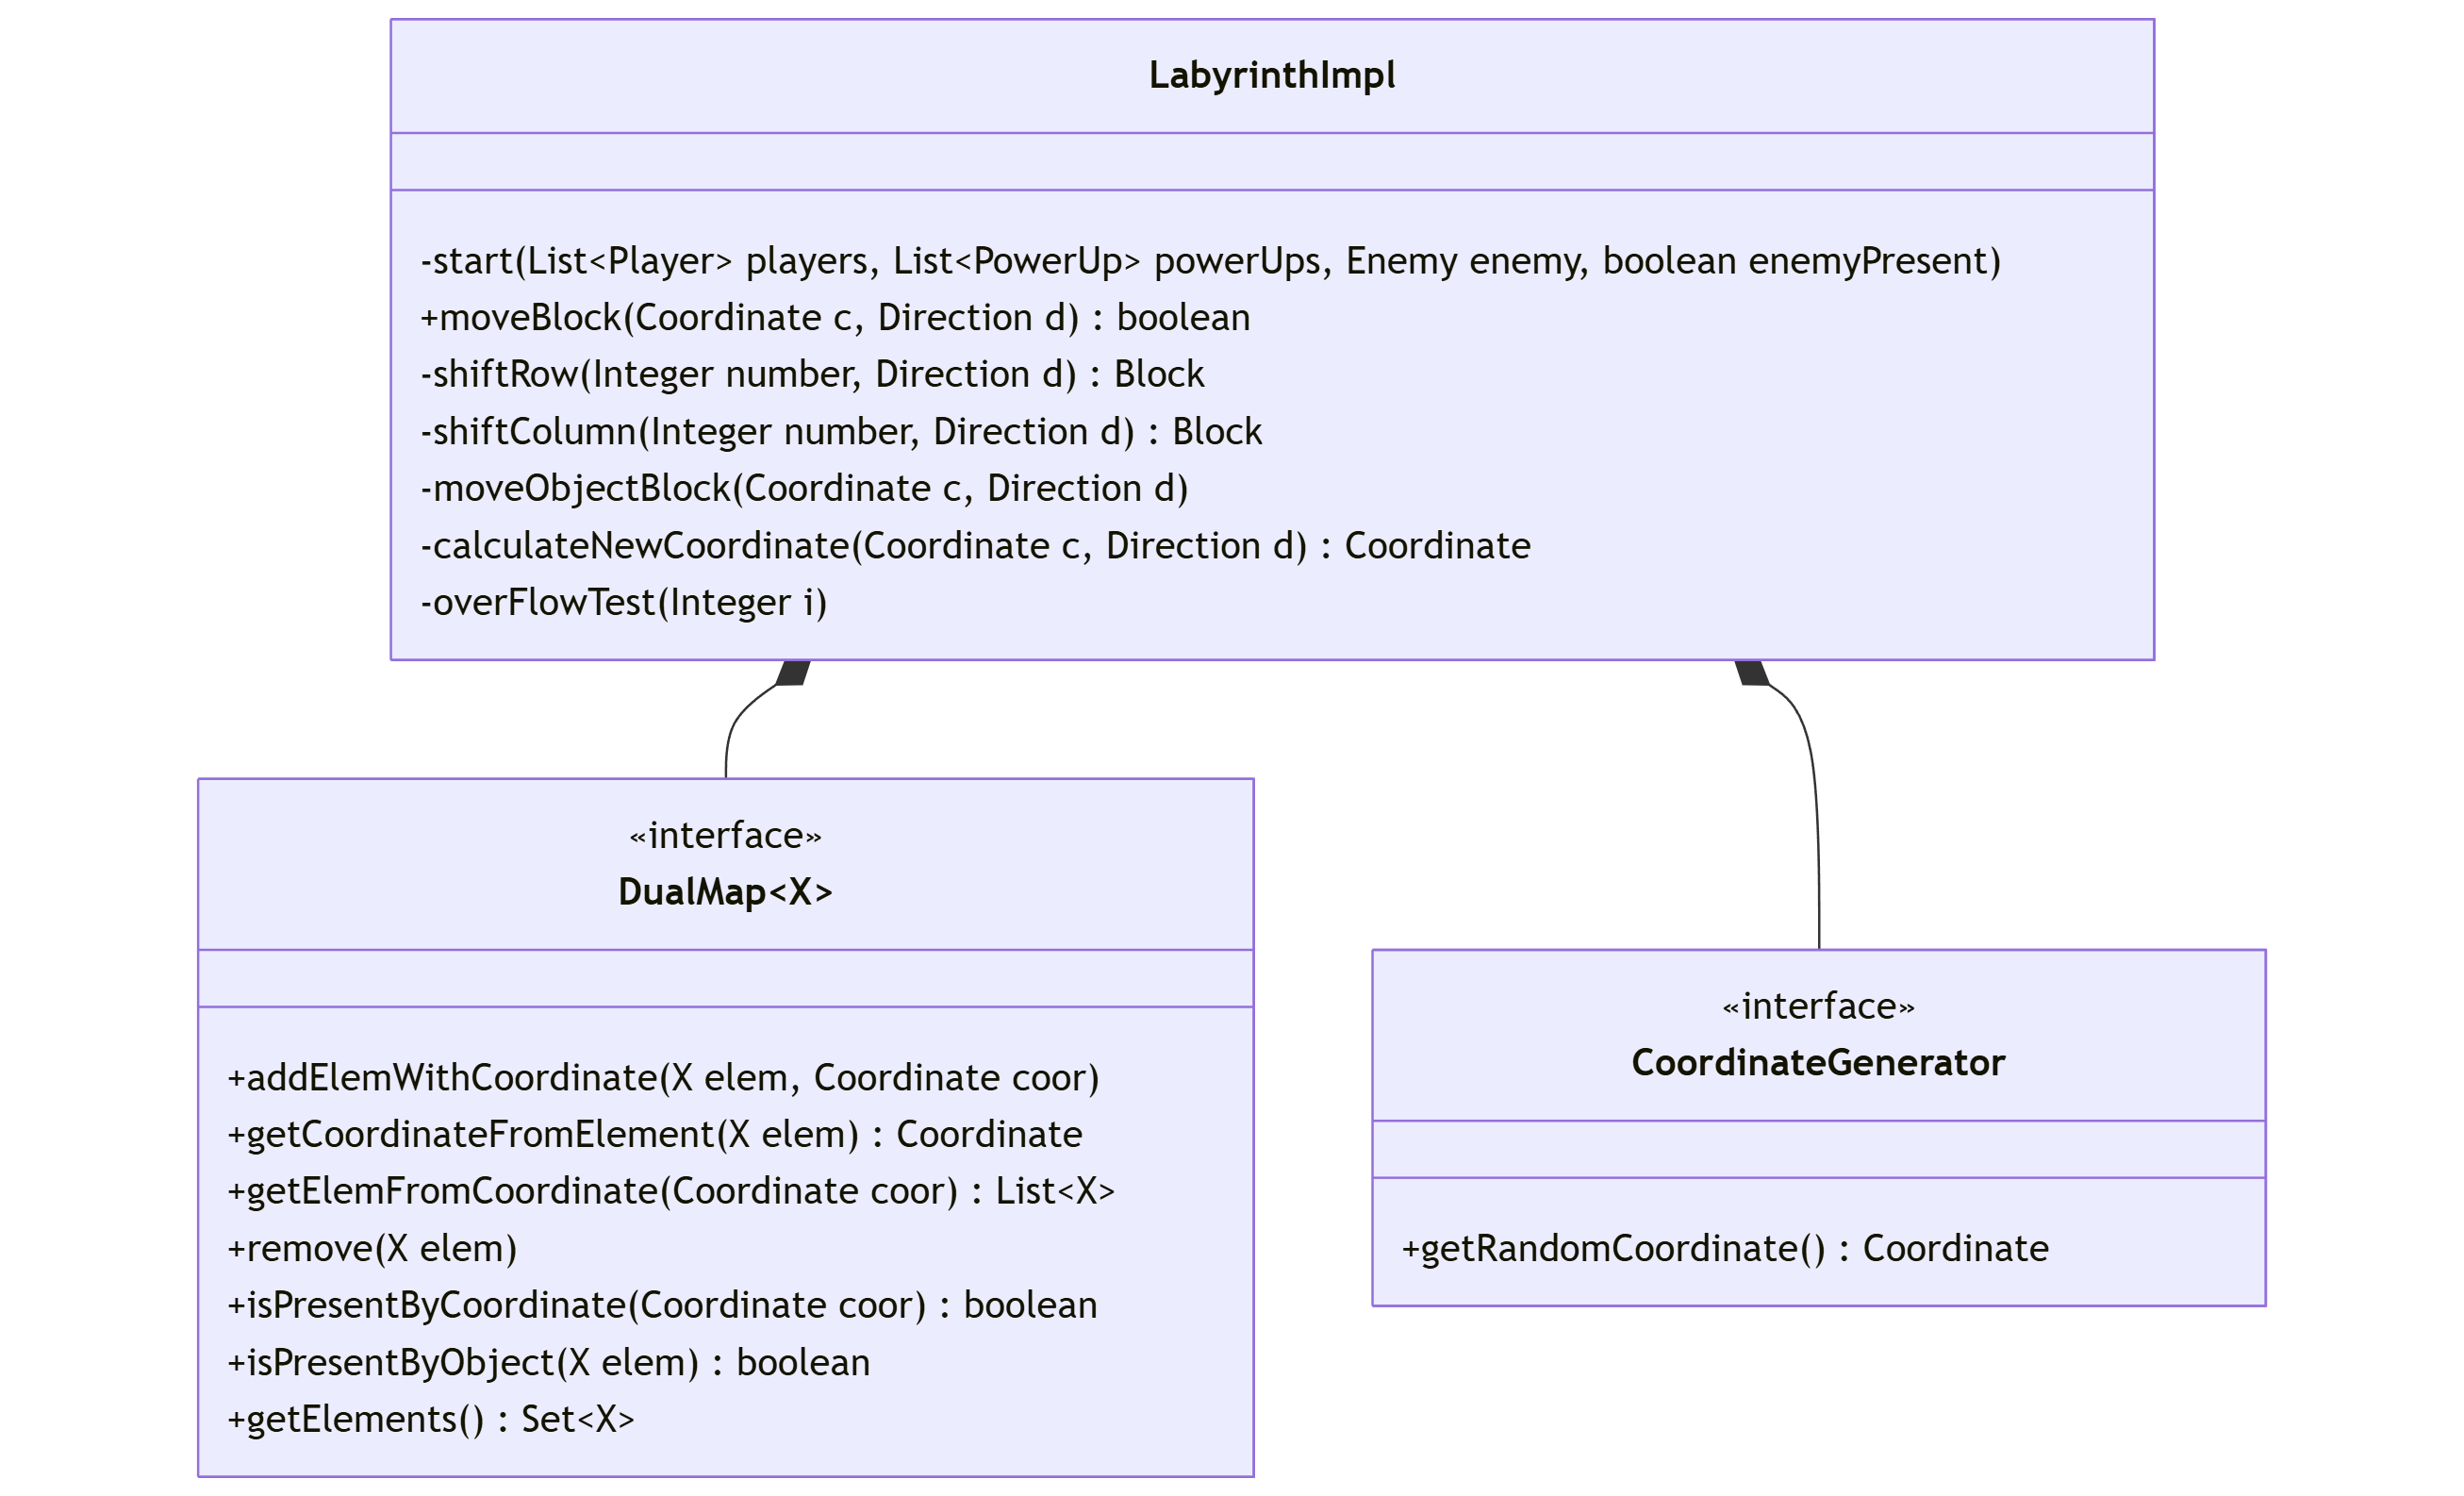
\includegraphics[width=14cm]{img/GestioneCoordinate.png}
	\caption{Schema UML del processo per la gestione delle coordinate}
	\label{img:Gestione Coordinate}
\end{figure}
\textbf{Caricamento immagini e disegno grafica}
\\
\\
\textbf{PROBLEMA}
Nel contesto del gioco ispirato al Labirinto Magico, è essenziale offrire all’utente una rappresentazione grafica chiara, coerente e reattiva dello stato di gioco. 
La visualizzazione deve adattarsi dinamicamente alle dimensioni della finestra e 
riflettere fedelmente ogni modifica del modello, inclusi la rotazione delle tessere, la posizione dei giocatori, la presenza di obiettivi o nemici.
\\
\\
\textbf{SOLUZIONE}
Per affrontare questo problema ho adottato una chiara separazione tra la logica di visualizzazione e rendering grafico.
In particolare la soluzione che ho adottato utilizza 3 componenti.
\begin{itemize}
	\item \textbf{DrawPanel}: componente di basso livello incaricato esclusivamente del disegno su schermo. Riceve una lista strutturata di elementi grafici già processati e li renderizza.
	\item \textbf{LogicDrawPanel}: componente intermedio creato dal DrawPanel che si occupa della logica di visualizzazione. 
	Analizza lo stato del modello (GameController), calcola le coordinate pixel, la rotazione e la dimensione ottimale per ogni immagine da disegnare.
	\item \textbf{ImageLoader}:  classe dedicata al caricamento e alla gestione delle risorse grafiche. Associa ogni elemento di gioco alla sua rispettiva immagine.
\end{itemize}
Quando la GameView richiede un aggiornamento:
\begin{itemize}
	\item Il DrawPanel interroga il LogicDrawPanel.
	\item Il LogicDrawPanel analizza lo stato corrente del gioco e costruisce più elementi contenenti tutte le informazioni utili per il rendering.
	\item Il DrawPanel renderizza tale rappresentazione.
\end{itemize}
Il calcolo delle proporzioni avviene dinamicamente in base alla dimensione della finestra dell’applicazione, garantendo un’interfaccia responsive. 
In fondo a tutto ciò ho anche deciso di aggiungere per ogni giocatore un'immagine uguale al suo personaggio ma cambiata di colore per indicare graficamente, 
il giocatore che sta svolgendo il turno.
\\
\\
\textbf{PRO}
\begin{itemize}
	\item La separazione tra logica e rendering consente una maggiore manutenibilità e una lettura più chiara del codice.
	\item L'interfaccia utente si adatta automaticamente alla risoluzione della finestra.
	\item Si possono aggiungere facilmente nuove funzionalità grafica o set di elementi senza dover apportare modifiche al codice già implementato.
\end{itemize}
\textbf{CONTRO}
\begin{itemize}
	\item In caso di aggiornamento del model il LogicDrawPanel si deve ricalcolare tutti gli elementi anche quelli non modificati di posizione o rotazione.
\end{itemize}
\begin{figure}[H]
	\centering{}
	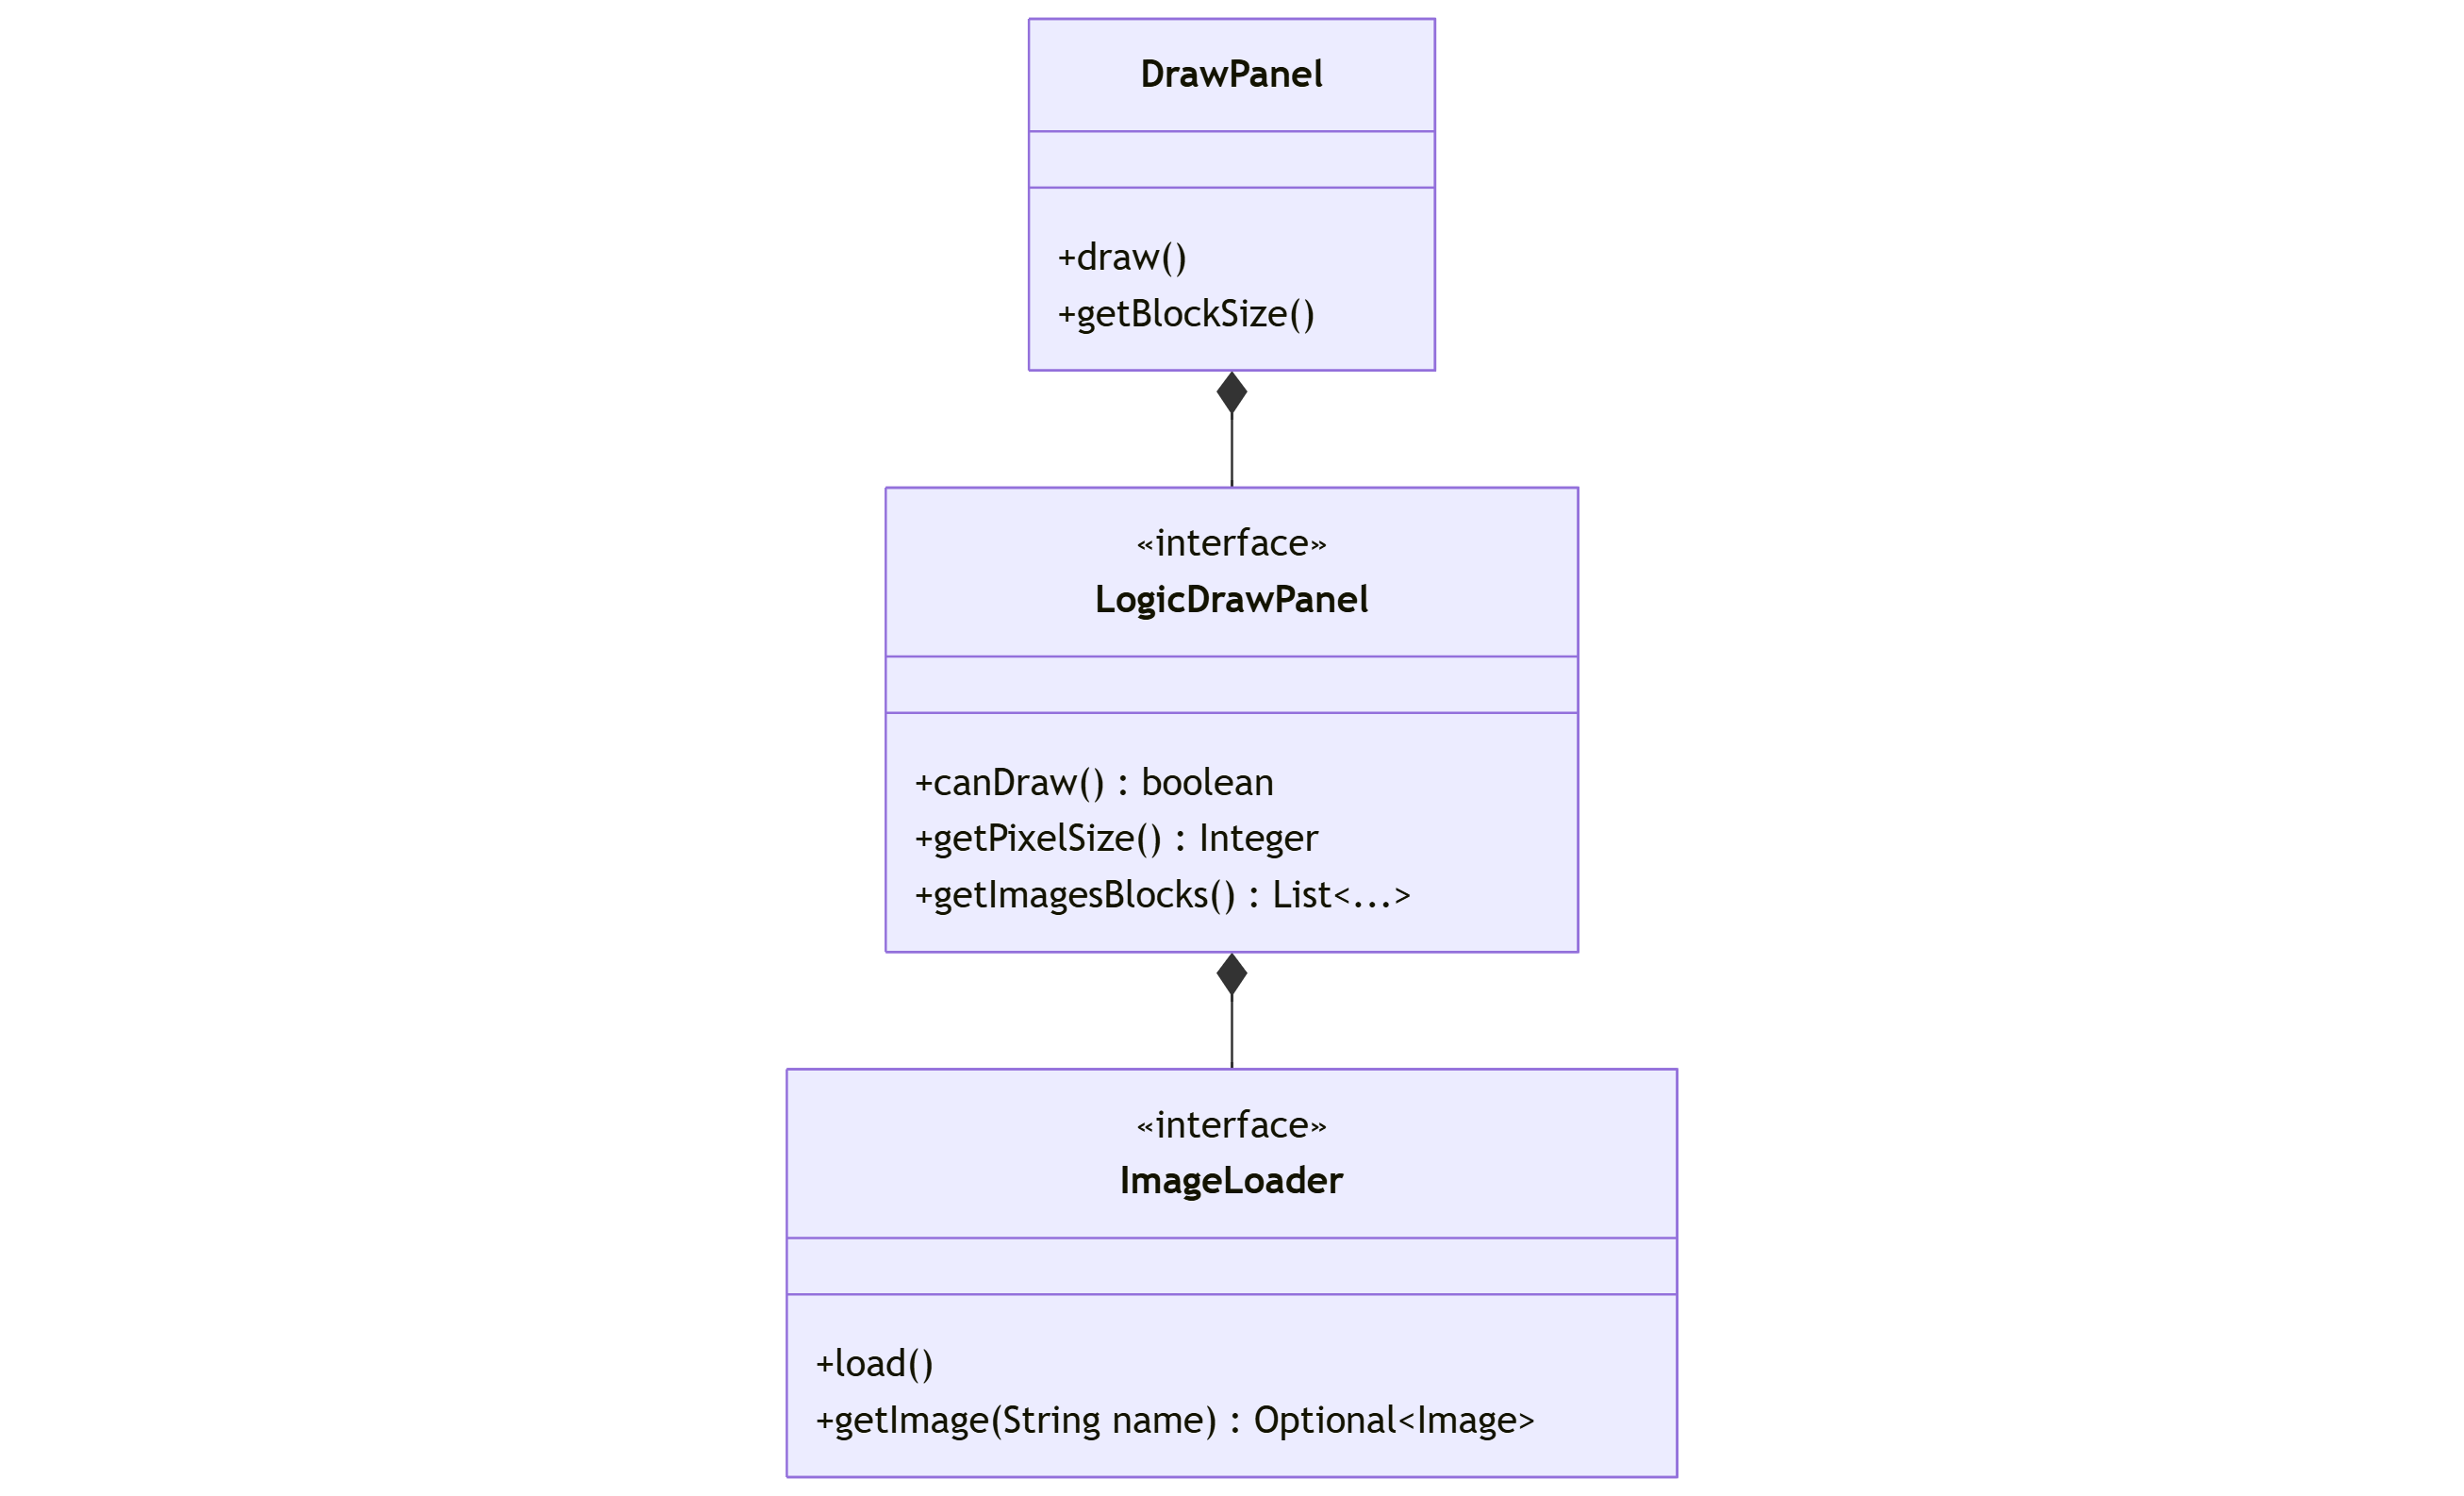
\includegraphics[width=14cm]{img/DisegnareGrafica.png}
	\caption{Schema UML del processo per aggiornare la grafica di gioco}
	\label{img:Aggiornamento Grafica}
\end{figure}
\textbf{Metodi per la gestione dei punteggi, nomi e informazioni}
\\
\\
\textbf{PROBLEMA}
Durante lo svolgimento della partita, è fondamentale fornire al giocatore un feedback continuo sullo stato del gioco. In particolare, è necessario visualizzare:
\begin{itemize}
	\item A chi tocca il turno corrente.
	\item Qual è l’azione richiesta.
	\item I power-up utilizzabili per ciascun giocatore.
	\item Il vincitore della partita (quando rilevante).
	\item Una classifica aggiornata dei giocatori con informazioni sul punteggio e lo stato.
\end{itemize}
Queste informazioni devono essere rese accessibili in modo intuitivo e integrato nell’interfaccia utente, 
senza legare la logica della visualizzazione direttamente al modello del gioco.
\\
\\
\textbf{SOLUZIONE}
Per separare correttamente la logica del gioco dalla logica di presentazione, è stata introdotta una componente intermedia: la \textbf{LogicGameView}.
In questa classe io ho creato delle funzionalità per la trasformazione di informazioni dal model in stringe comprensibili dall'utente e mostrabili dalla view.
Tra queste ci sono:
\begin{itemize}
	\item Turni e azioni: restituisce il nome del giocatore a cui tocca e la descrizione dell’azione da compiere.
	\item Power-Up: crea e restituisce una lista dei power-up attivi utilizzabili da un giocatore, da mostrare tramite ComboBox.
	\item Esito della partita: genera un messaggio da visualizzare alla fine del gioco, indicando il vincitore.
	\item Classifica giocatori: restituisce, per ciascun giocatore, una stringa contenente nome, punteggio e stato.
\end{itemize}
\textbf{PRO}
\begin{itemize}
	\item Separazione delle responsabilità: La logica trasforma i dati e li passa alla view rendendosi intermediaria tra l'interfaccia utente e il model.
	\item Manutenibilità: In caso di future modifiche alla stringhe da visualizzare si possono cambiare codici poco complessi e distaccati dalla view quindi di facile elaborazione.
	\item Flessibilità: in caso di necessità queste informazioni possono essere mostrate dalla view in modi differenti senza dover ricorrere a un ricalcolo delle stringhe.
\end{itemize}
\textbf{CONTRO}
\begin{itemize}
	\item Bisogna dare paricolare attenzione agli aggiornamenti della view perché in caso di cambiamento del model ma non della view si prensenta per l'utente della confusione 
	nello stato della partita.
\end{itemize}
\begin{figure}[H]
	\centering{}
	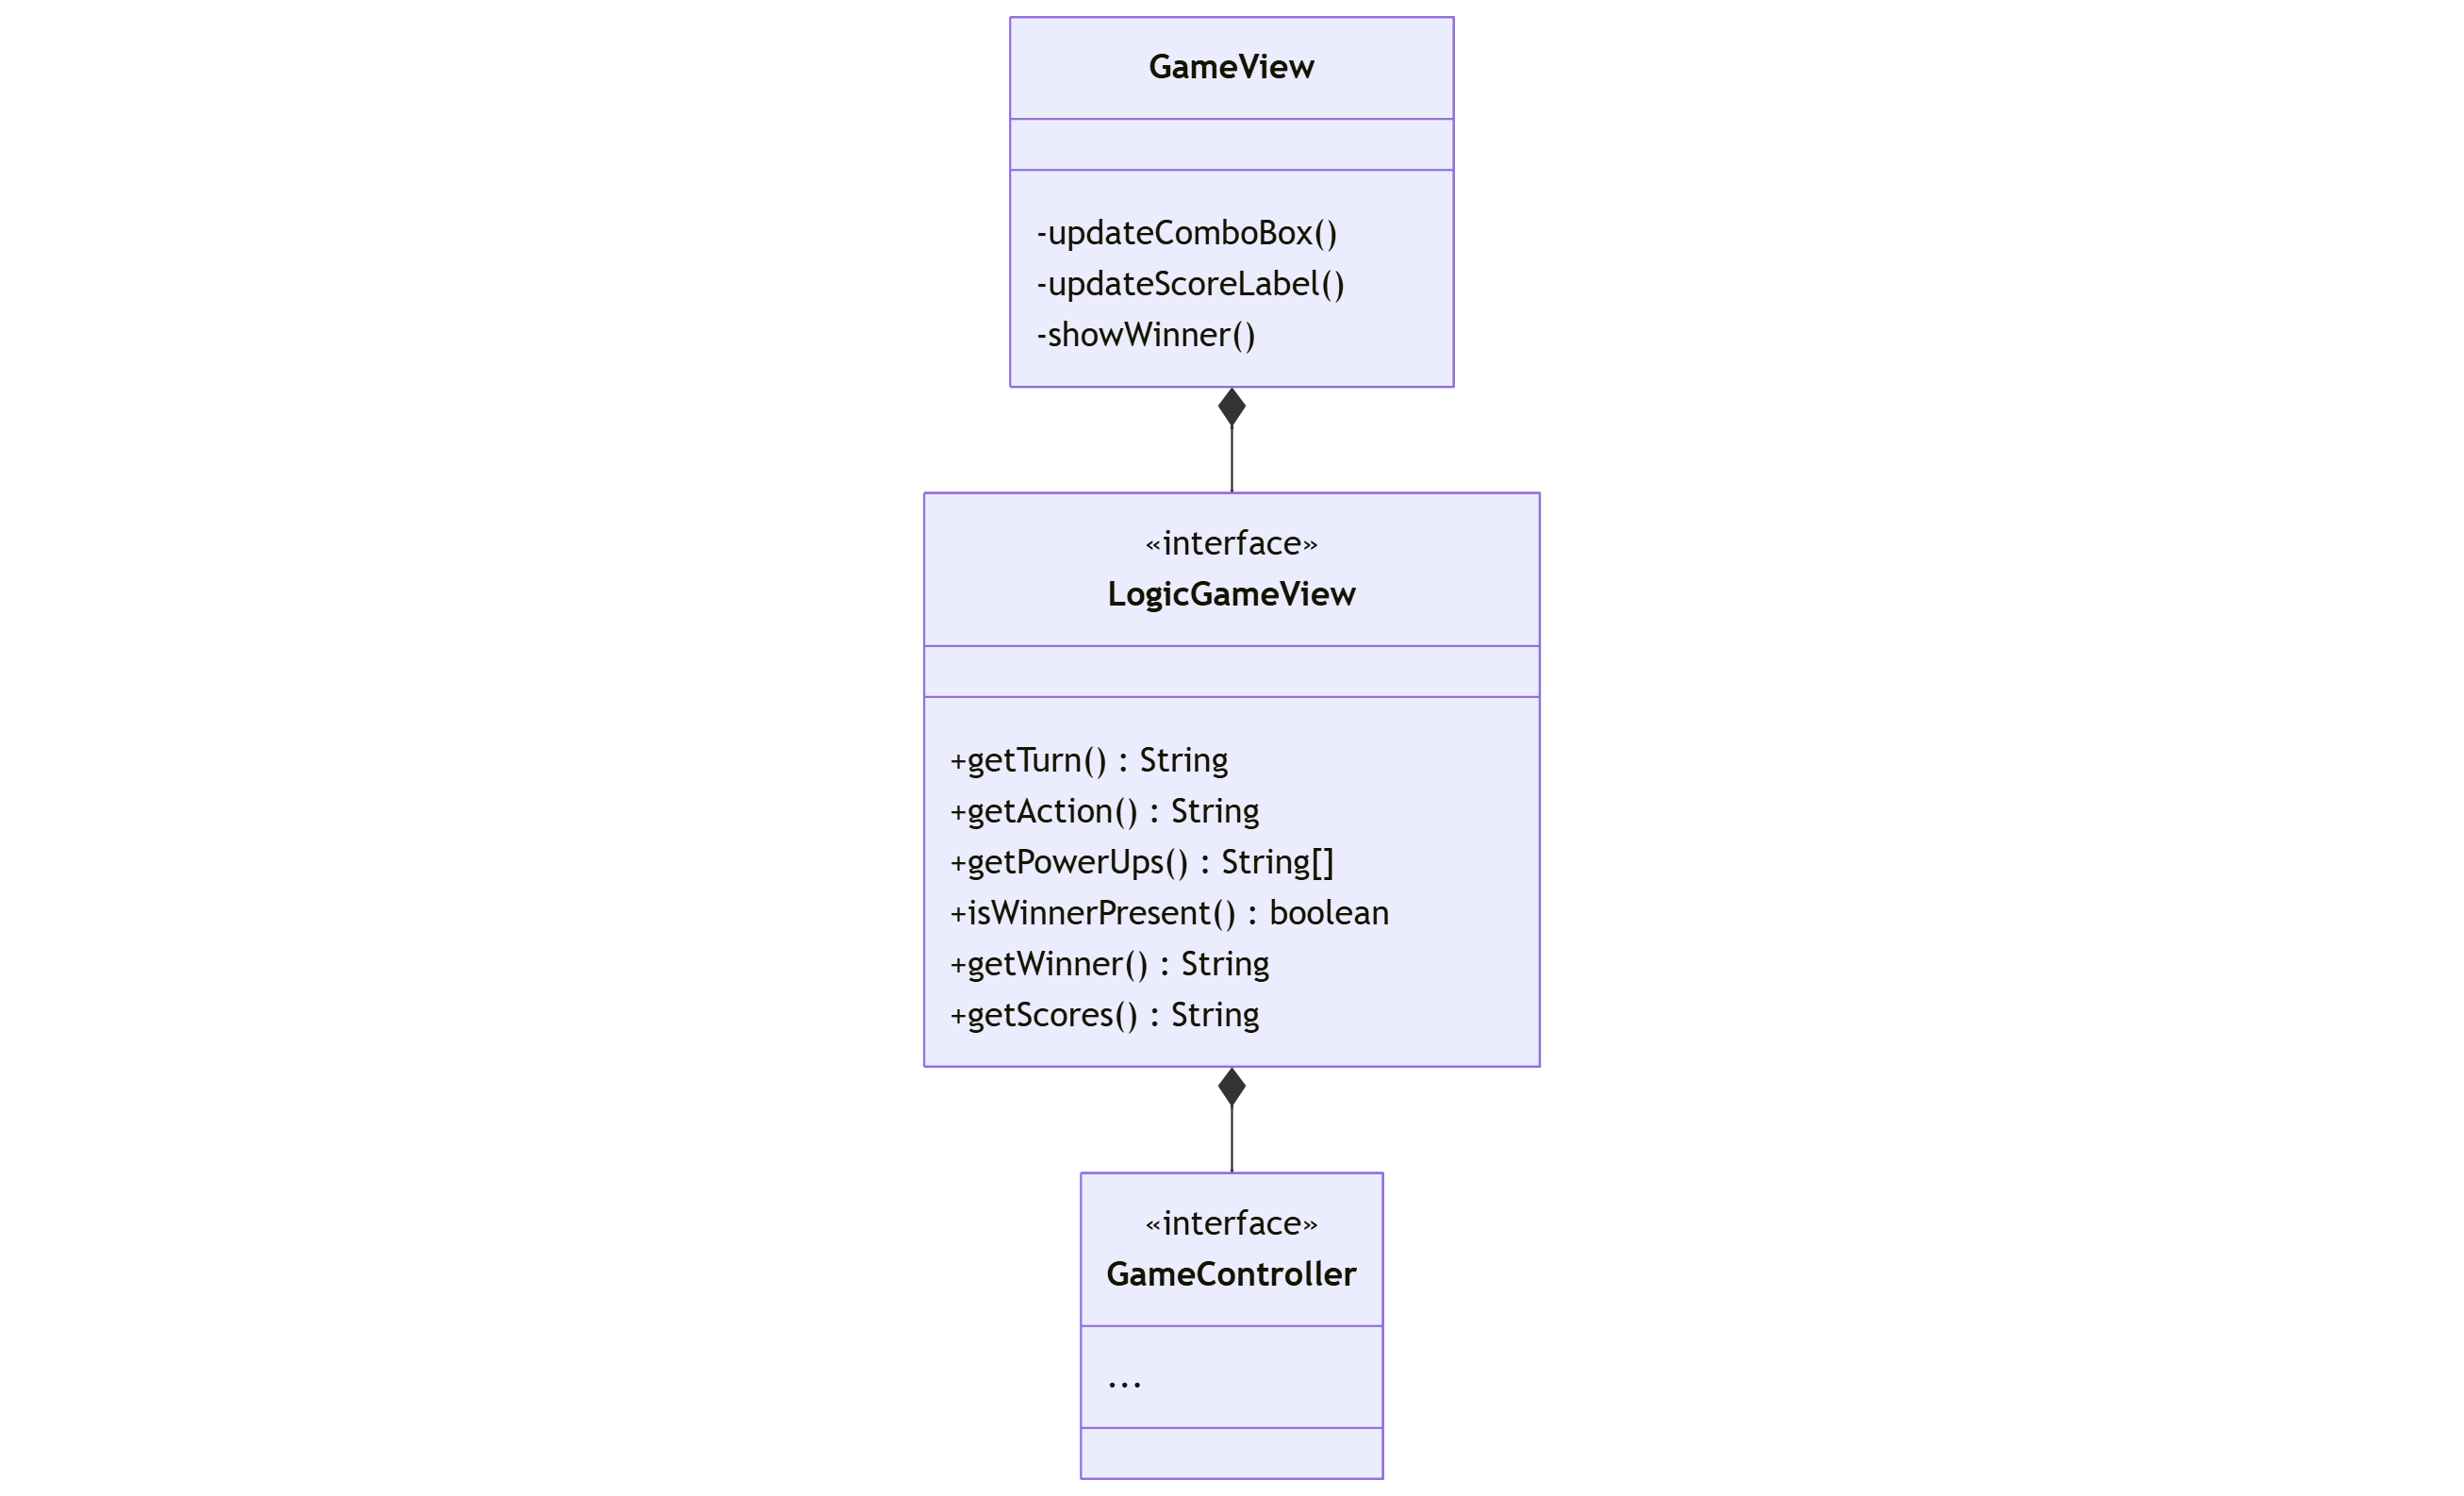
\includegraphics[width=14cm]{img/TraduzioneInformazioni.png}
	\caption{Schema UML dei processi per leggere le informazioni dal gioco}
	\label{img:Traduzione Informazioni}
\end{figure}

\newpage
\subsection{Stefano Baiano}
\textbf{Gestione delle collisioni}
\\
\\
\textbf{PROBLEMA}
\\
Quando un personaggio deve muoversi bisogna verificare che ci sia un'apertura nel labirinto dove il personaggio
desidera muoversi. Inoltre anche il nemico deve poter verificare le stesse condizioni del giocatore.
\\
\\
\textbf{SOLUZIONE}
\\
Per riuscire a gestire la verifica di collisioni è stata creata una classe che verificano se esiste un'entrata nella direzione desiderata. 
Per capire quali caselle sono da controllare viene usata un'altra classe per non sovraccaricare la prima:
\begin{itemize}
	\item DirectionCheck - classe che controlla se esiste una entrata in una specifica direzione di una casella. In caso affermativo restituisce true, altrimenti false.
	\item ActionPredicate - Prende le azioni passate dall'ActionController e capisce quali caselle sono da controllare. In caso l'azione sia fattibile restituisce true, altrimenti false.
\end{itemize}
\textbf{PRO}
\\
\begin{itemize}
	\item Facile utilizzo: la classe rimane semplice da utilizzare in quanto con le funzioni intuitive permette di controllare tutte le direzioni
	in poche semplici parole. Es: playerCanMove(player, direction, labyrinth) checkLeftEntrance(coord, direction)
\end{itemize}
\textbf{CONTRO}
\\
\begin{itemize}
	\item Complessa lettura del codice: visto il facile utilizzo i vari processi devono essere effettuati dalla classe principale. 
	Per questo la lettura del codice risulta non intuitiva.
\end{itemize}
\begin{figure}[H]
	\centering{}
	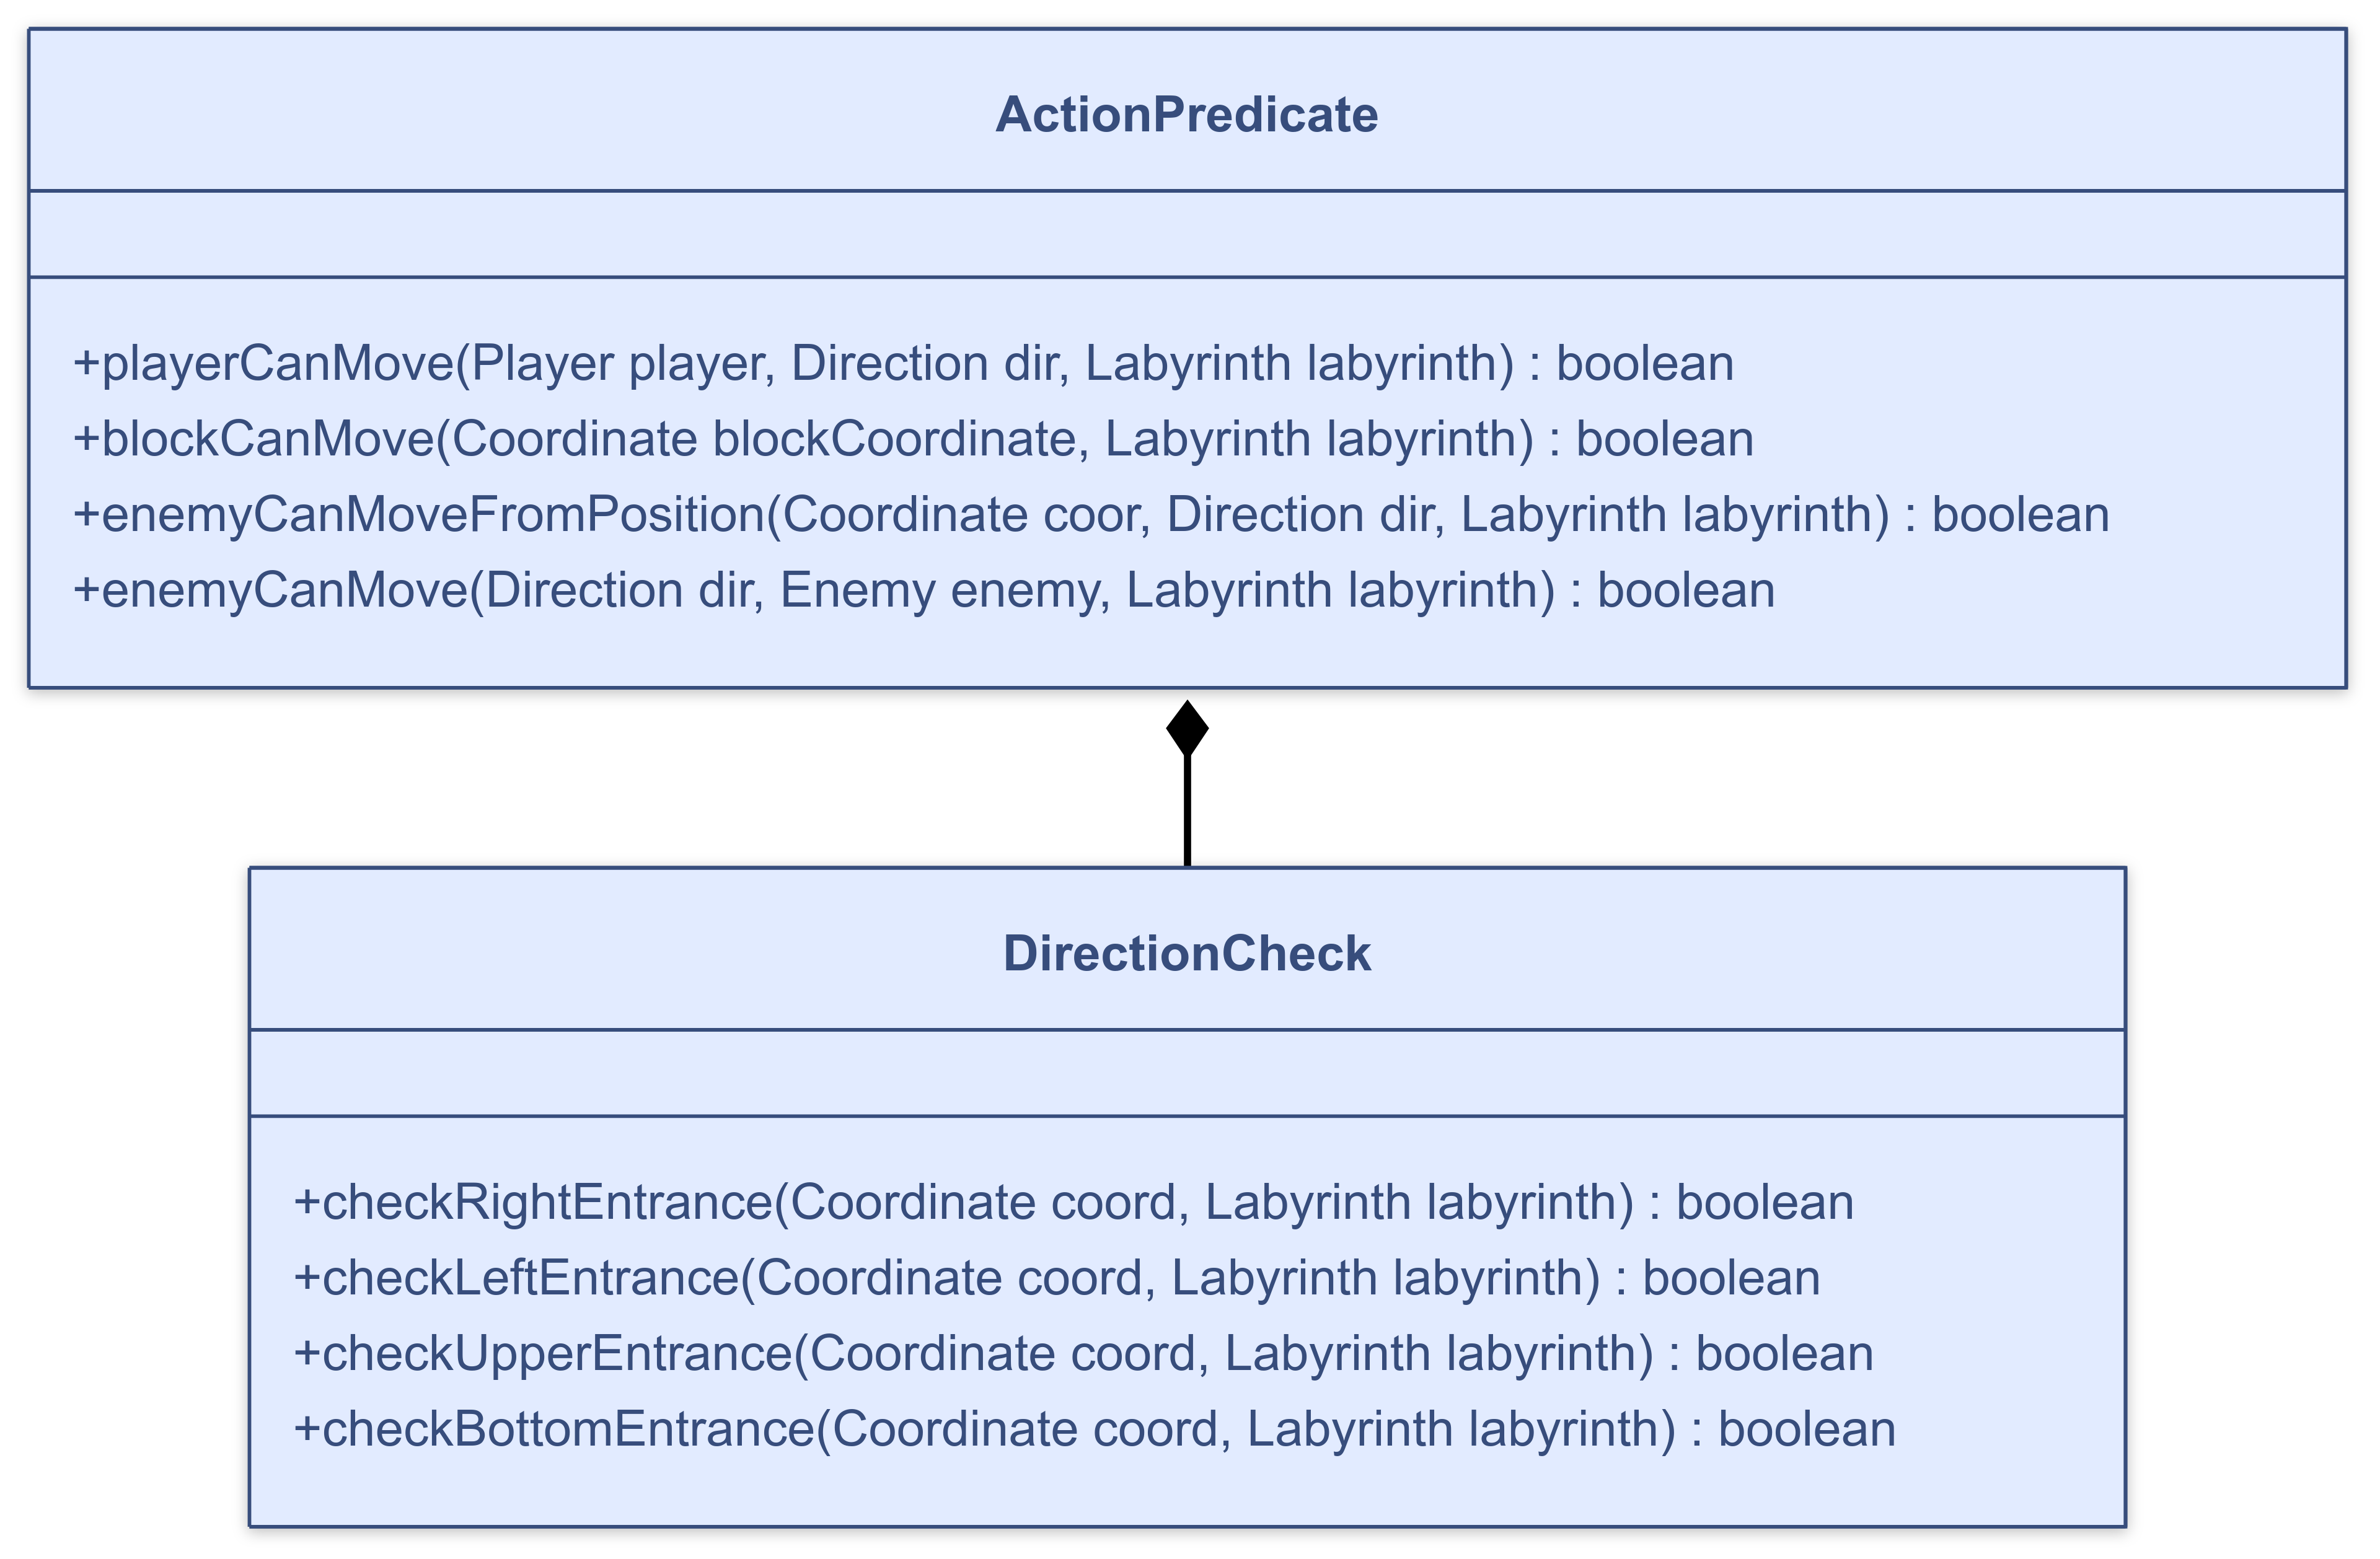
\includegraphics[width=10cm]{img/GestioneCollisioni.png}
	\caption{Schema UML delle due classi per la gestione collisioni}
	\label{img:GestioneCollisioni}
\end{figure}
\textbf{Gestione gioco}
\\
\\
\textbf{PROBLEMA}
\\
Bisogna creare una struttura che gestisce gli input dalla gameView e che faccia da tramite per le varie classi che 
sono state create all'interno del labirinto.
\\
\\
\textbf{SOLUZIONE}
\\
Per sistemare a questa problematica è stata creata una classe, ActionController, con l'obiettivo di coordinare le varie informazioni che vengono da 
altre classi condividendo i dati tra le varie strutture:
\begin{itemize}
	\item Controlli delle azioni: Legge le azioni che arrivano dalla view e le traduce. Usa l'ActionPredicate per capire se è fattibile l'azione.
	\item Cambiamento dei dati: se l'azione è effettuabile vengono cambiati i dati tramite la classe Labyrinth e TurnManager.
\end{itemize}
\textbf{PRO}
\\
\begin{itemize}
	\item Gestione subordinata: La gestione delle varie azioni è gestita ognuna da sottoclassi che svolgono poche semplici azioni che permettono una
	fruibilità del codice elevata.
	\item Flessibilità: In caso si vogliano aggiungere azioni nuove il codice rimane molto semplice per permettere queste aggiunte.
\end{itemize}
\textbf{CONTRO}
\begin{itemize}
	\item Nel caso di problemi o errori per sistemarlo bisogna controllare tante classi diverse tra loro che gestiscono diversi dati. E' quindi 
	molto semplice perdersi nel codice.
\end{itemize}
\begin{figure}[H]
	\centering{}
	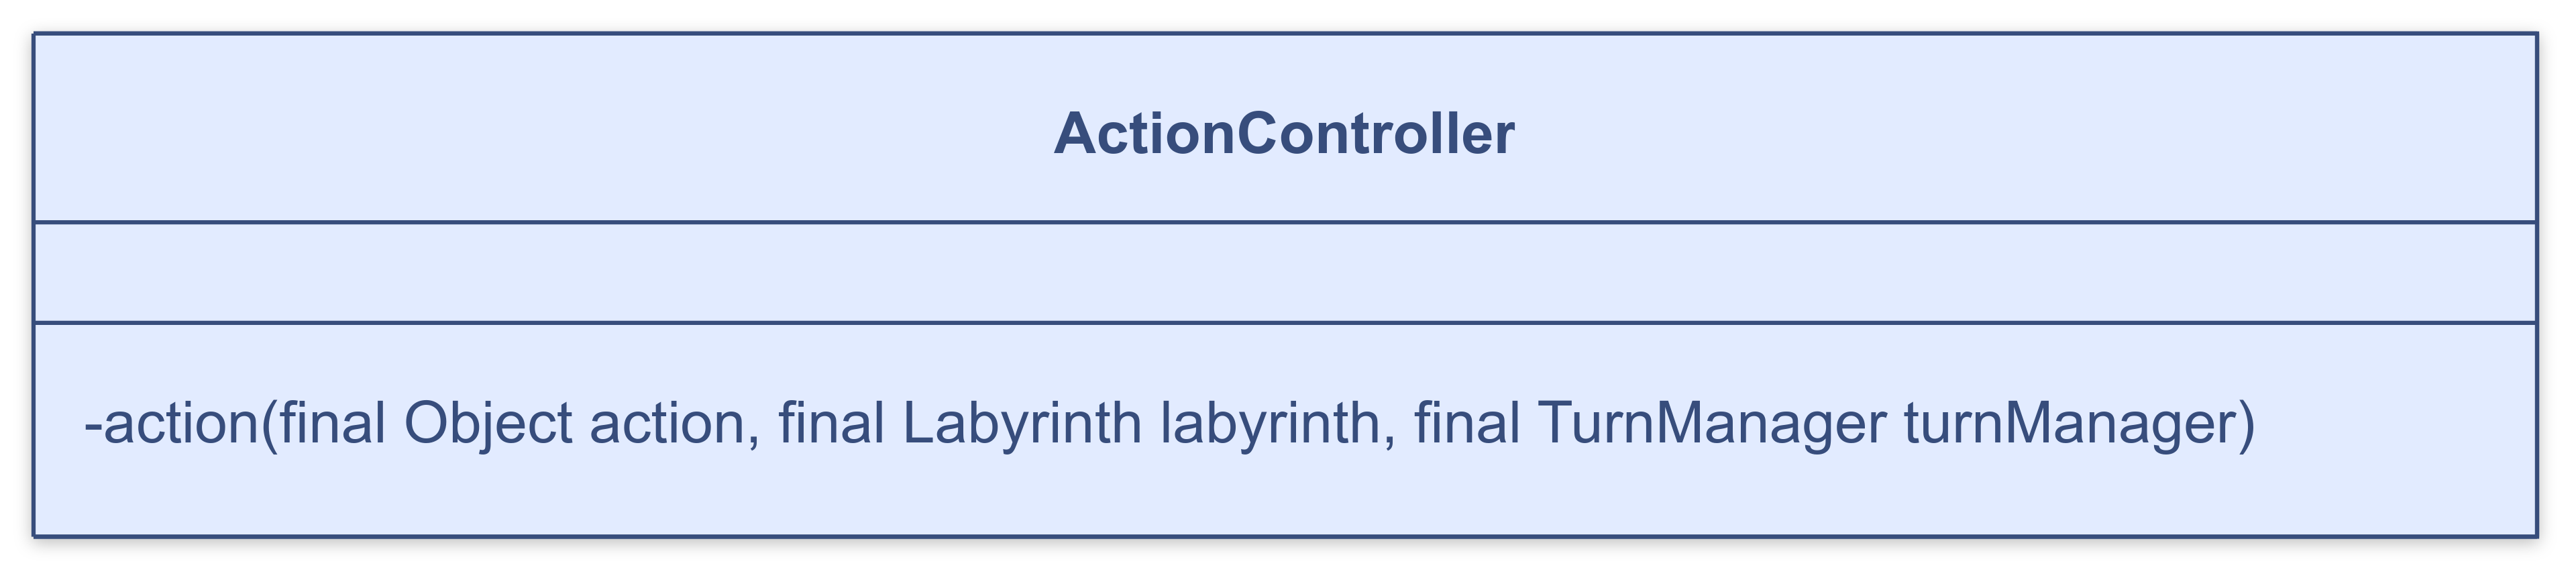
\includegraphics[width=12cm]{img/ActionController.png}
	\caption{ActionController con la sua funzione che permette di far funzionare le azioni del gioco}
	\label{img:ActionController}
\end{figure}
\textbf{Gestione dei salvataggi}
\\
\\
\textbf{PROBLEMA}
\\
Il gioco necessita di un sistema di salvataggio, ed il corrispettivo caricamento, di una partita. Per farlo è entrata la problematica 
della Serialization che impedisce l'uso dei vari Optional in quanto non sono serializzabili secondo la classe Serialization.
\\
\\
\textbf{SOLUZIONE}
\\
Per riuscire a risolvere la problematica sono state rese tutte le classi Serializable e dove comparivano Optional che andavano salvati, ad esempio 
nella prima versione dell'Enemy, è stata creato un Pair di boolean ed Enemy per poter riconoscere se esiste o meno il nemico.
Vengono ora implementate due classi, una per il salvataggio, che verrà richiamata dal GameController, e l'altra per il caricamento, che verrà richiamata dal MainMenuController.
\\
\\
\textbf{PRO}
\begin{itemize}
	\item Si riesce con molta facilità ad aggiungere nuove classi ai salvataggi/caricamenti aggiungendo Serializable vicino 
	alla classe e passando al SaveController per poter effettuare il salvataggio.
\end{itemize}
\textbf{CONTRO}
\begin{itemize}
	\item Non si può utilizzare la classe Optional, utile per molte funzioni che sono più lunghe e complesse per via del Pair creato.
\end{itemize}
\begin{figure}[H]
	\centering{}
	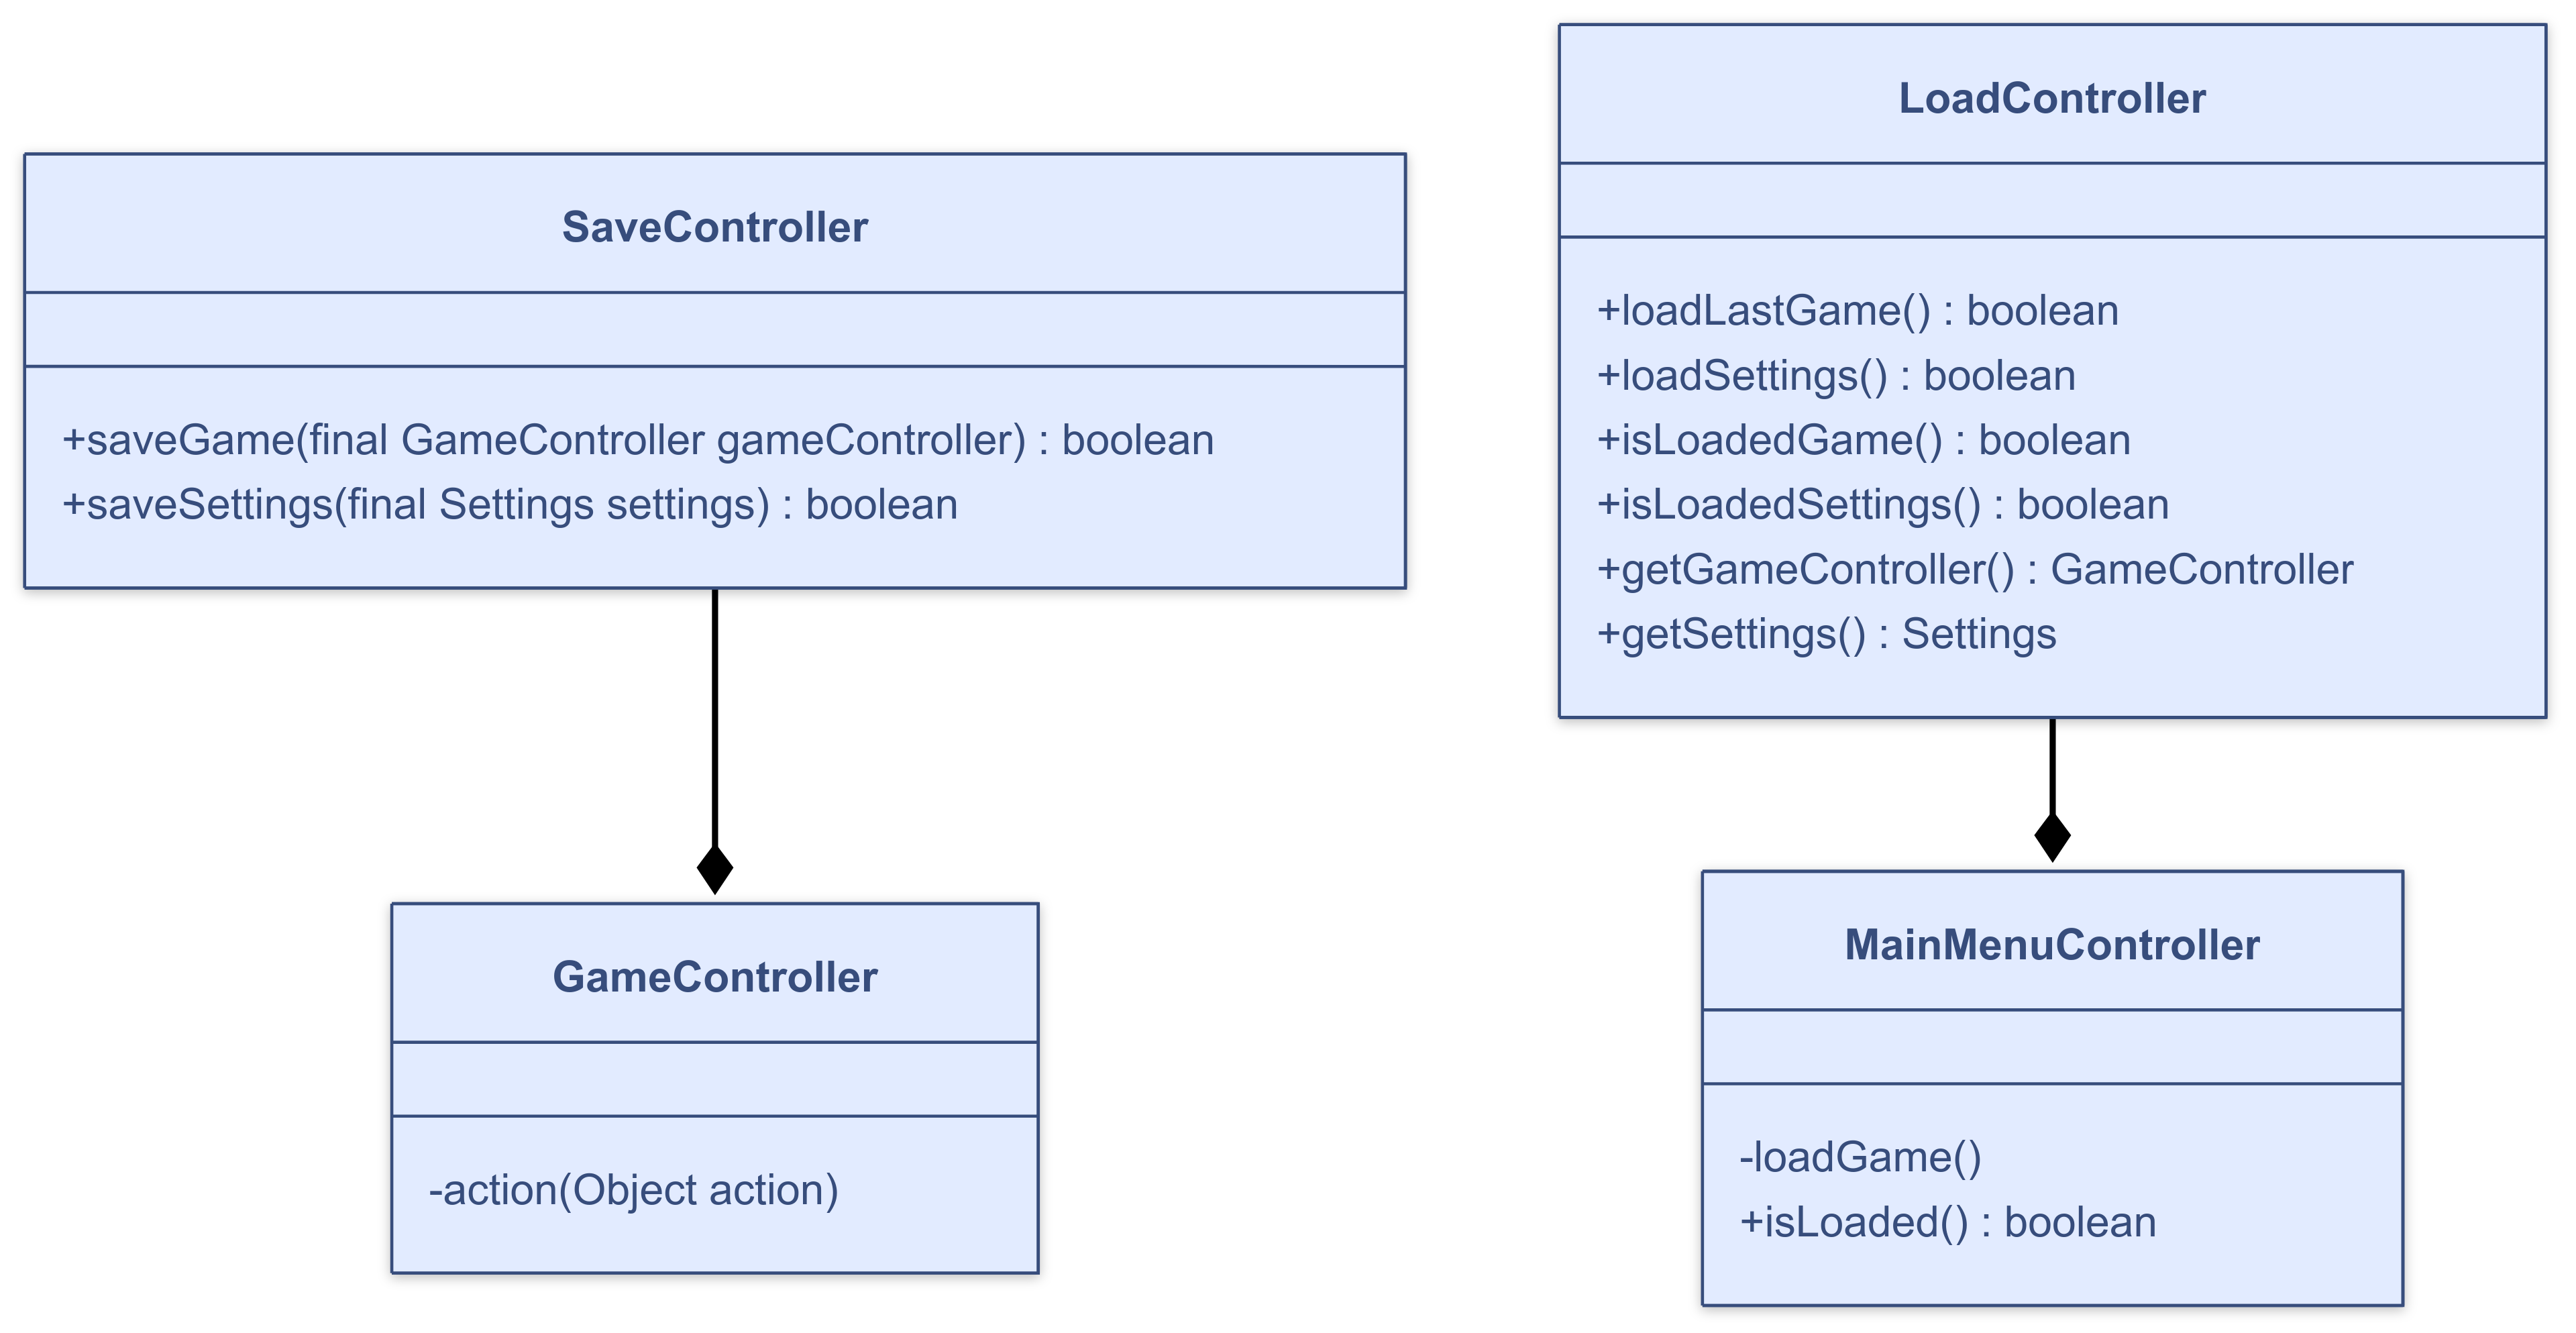
\includegraphics[width=\textwidth]{img/Saving.png}
	\caption{Schema UML di salvataggio e caricamento}
	\label{img:saving}
\end{figure}
\newpage
\subsection{Andrea Monti}
\textbf{Movimento del nemico}
\\
\\
\textbf{PROBLEMA}
Creare un layer di astrazione minimale che permetta di far muovere il nemico alla posizione successiva in base a una certa logica, 
senza esporre i dettagli implementativi sottostanti.
\\
\\
\textbf{SOLUZIONE}
Creazione di un’interfaccia EnemyAI con un singolo metodo getNextPosition() che restituisce la 
prossima posizione del nemico (ogni tipologia specifica di AI avrà ovviamente una diversa implementazione). 
Di seguito i dettagli relativi a ciascuna delle tre implementazioni:
\begin{itemize}
	\item \textbf{SingleStepRandomAI}: effettua un solo passo in una direzione casuale. 
	\item \textbf{RandomAI}: muove il nemico per un numero casuale di passi (tra 2 e 5), scegliendo ogni volta una 
	direzione casuale valida e aggiungendo ogni nuova posizione alla lista che viene restituita.
	\item \textbf{ChaseAI}: è la più complessa e calcola il percorso più breve verso il giocatore.
	Ciò avviene tramite una BFS, generando tutte le celle raggiungibili dal nemico e cercando tra queste la posizione 
	di un giocatore. Se esiste un percorso verso tale giocatore, viene restituita la sequenza di coordinate che rappresentano 
	il cammino verso di lui; se invece non esiste alcun percorso verso nessun giocatore, si limita a restituire la posizione 
	attuale o si affida a una mossa casuale tramite SingleStepRandomAI.
\end{itemize}
\begin{figure}[H]
	\centering{}
	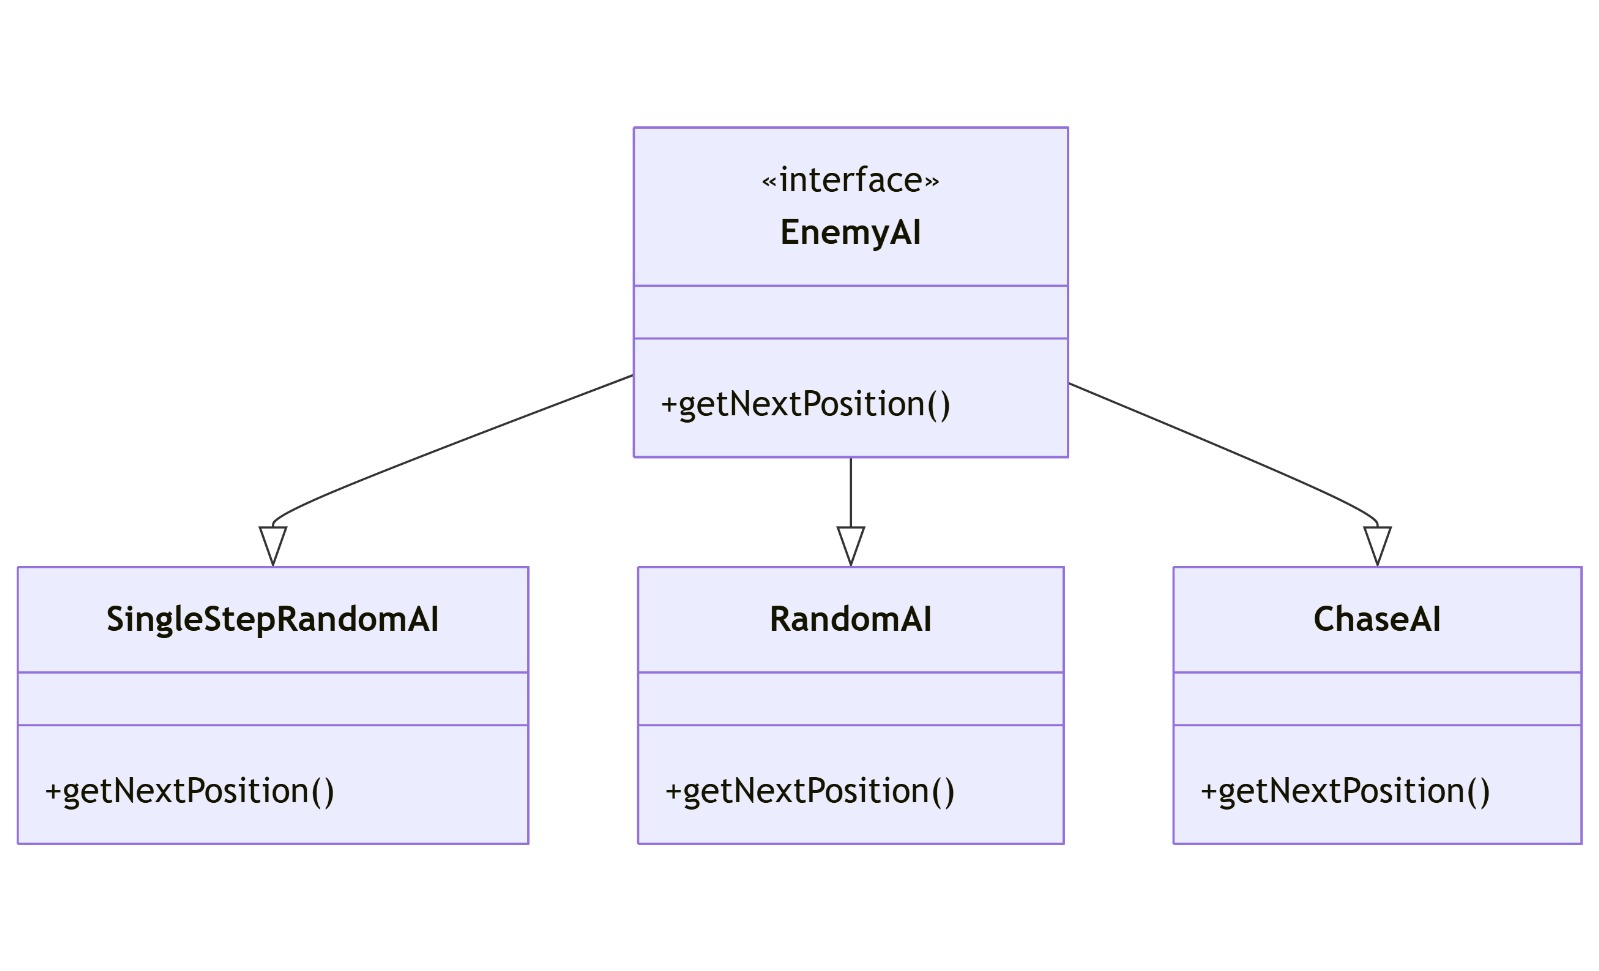
\includegraphics[width=14cm]{img/MovimentoNemico.png}
	\caption{Schema UML del processo per il movimento del nemico}
	\label{img:Movimento Nemico}
\end{figure}
\textbf{Gestione dei nemici con il pattern Factory}
\\
\\
\textbf{PROBLEMA}
Occorre creare un sistema in grado di istanziare il nemico con un’AI diversa a seconda della difficoltà di gioco scelta.
\\
\\
\textbf{SOLUZIONE}
Inizialmente ho pensato di implementare il sistema tramite classi astratte, ma poi l’idea è stata abbandonata in favore 
dell’utilizzo del pattern Factory, che ha reso più semplice e immediato il processo di creazione delle varie tipologie di nemici.
Con questo approccio si facilita anche l’estensibilità ed è possibile aggiungere nuovi tipi di nemici senza dover modificare 
il codice esterno. Inoltre, la classe Enemy è serializzabile, poiché nel gioco è presente un sistema di salvataggio.
L’interfaccia Enemy include metodi per tenere traccia dell’ultimo giocatore colpito: finché il nemico non cambia bersaglio o 
non torna il turno di quel giocatore, potrebbe continuare a colpirlo senza però sottrargli ulteriori PowerUp.
\begin{figure}[H]
	\centering{}
	\includegraphics[width=14cm]{img/DifficoltàNemico.png}
	\caption{Schema UML del processo per le diverse difficoltà del nemico}
	\label{img:Pattern Factory}
\end{figure}
\noindent\textbf{Evitare la duplicazione del codice}
\\
\\
\textbf{PROBLEMA}
Fornire funzioni di supporto per il movimento dei nemici sulla griglia, favorendo il riuso di codice ed evitando duplicazioni.
\\
\\
\textbf{SOLUZIONE}
Applicando il principio DRY, ho creato una classe di utility MovementUtilities con metodi statici di supporto 
per il movimento dei nemici sulla griglia. Questa classe consente il riutilizzo di alcune logiche di movimento 
da parte delle varie intelligenze artificiali, evitando duplicazioni di codice.
La classe contiene due metodi statici principali. Il primo calcola la nuova coordinata in base a una posizione iniziale e
una direzione (su, giù, destra, sinistra), mentre il secondo traduce un intero (da 0 a 3) nella corrispondente direzione. 
\\
\\
\textbf{Gestione dei turni di gioco}
\\
\\
\textbf{PROBLEMA}
Creare un sistema in grado di gestire il flusso dei turni di gioco, stabilendo quale giocatore deve agire 
e quale azione deve compiere in ogni momento.
\\
\\
\textbf{SOLUZIONE}
Per gestire il flusso di gioco, ho creato una classe TurnManager che determina, per ciascuna fase di gioco, 
quale giocatore deve agire e quale tipo di azione può compiere. Ciò avviene tenendo traccia del giocatore attivo e 
dell’azione corrente (ad esempio, posizionamento di blocchi o movimento del giocatore).
Con questo sistema si garantisce che il gioco proceda in modo ordinato e che le azioni dei vari giocatori avvengano 
secondo la sequenza stabilita dalle regole.
\\
\\
\textbf{Creazione degli elementi di gioco}
\\
\\
\textbf{PROBLEMA}
Istanziare i vari elementi di gioco all’inizio della partita.
\\
\\
\textbf{SOLUZIONE}
Il metodo createMaze() nella classe BuilderImpl crea e restituisce un oggetto Labyrinth, inizializzando tutti i 
suoi componenti principali in base alle impostazioni fornite.
In base al numero di giocatori specificato, viene scelta la dimensione del labirinto: se i giocatori sono due, 
viene creato un labirinto più piccolo, mentre con tre o quattro giocatori si utilizza un labirinto più grande.
Prima della creazione del labirinto, il Builder utilizza dei metodi privati per generare i giocatori, i PowerUp 
e l’eventuale nemico (se specificato nelle impostazioni), per poi passarli al labirinto durante la sua inizializzazione.
\begin{figure}[H]
	\centering{}
	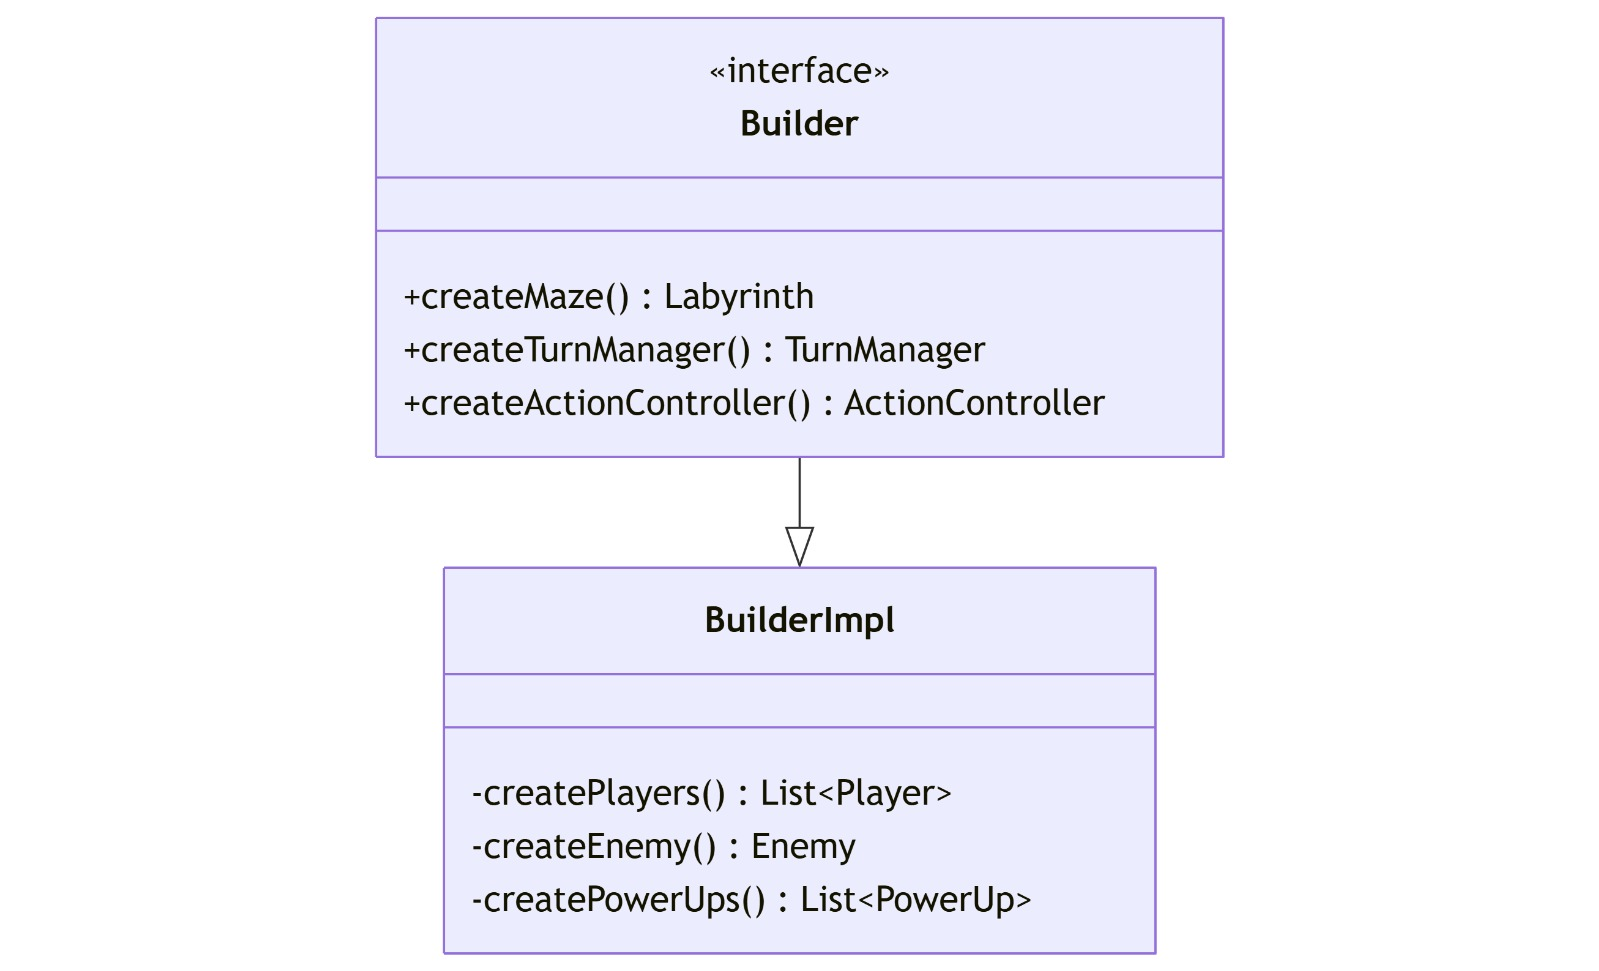
\includegraphics[width=14cm]{img/CreazioneElementi.png}
	\caption{Schema UML del processo per la creazione degli elementi di gioco}
	\label{img:Creazione Elementi}
\end{figure}

\newpage
\subsection{Simone Alocchi}

\subsubsection*{Gestione modulare dei Power-Up}

\paragraph{PROBLEMA}  
Nel gioco sono presenti molti tipi diversi di power-up, ciascuno con logiche differenti. Era necessario progettare un sistema che permettesse l'aggiunta semplice di nuovi power-up evitando ripetizione di codice, nel rispetto del principio DRY.

\paragraph{SOLUZIONE}  
Per gestire la presenza di molti tipi diversi di power-up, ho strutturato la logica seguendo i principi di riuso e facilità di estensione.  
Ho definito un’interfaccia \texttt{PowerUp} che stabilisce i metodi fondamentali che ogni power-up deve implementare, come \texttt{activate()}, oltre a metodi per la gestione dello stato (ad esempio se è stato raccolto o meno).
La classe astratta \texttt{PowerUpImpl} fornisce un’implementazione di base di questa interfaccia, occupandosi della logica comune a tutti i power-up: ad esempio, la gestione dell’identificativo, del nome e dello stato di raccolta.  
In questo modo, le sottoclassi possono concentrarsi solo sulla logica specifica del proprio effetto.
Ogni power-up concreto (come \texttt{SwapPositionPowerUp} o \texttt{InvulnerabilityPowerUp}) estende \texttt{PowerUpImpl} e ridefinisce il metodo \texttt{activate()} per implementare il proprio comportamento particolare.  
Questo approccio permette di aggiungere facilmente nuovi power-up senza duplicare codice, mantenendo la coerenza nella gestione del ciclo di vita e dell’interazione con il player.
In sintesi, la logica condivisa è centralizzata in \texttt{PowerUpImpl}, mentre la personalizzazione avviene nelle sottoclassi, rendendo il sistema robusto, estendibile e facile da mantenere.
\begin{figure}[H]
	\centering{}
	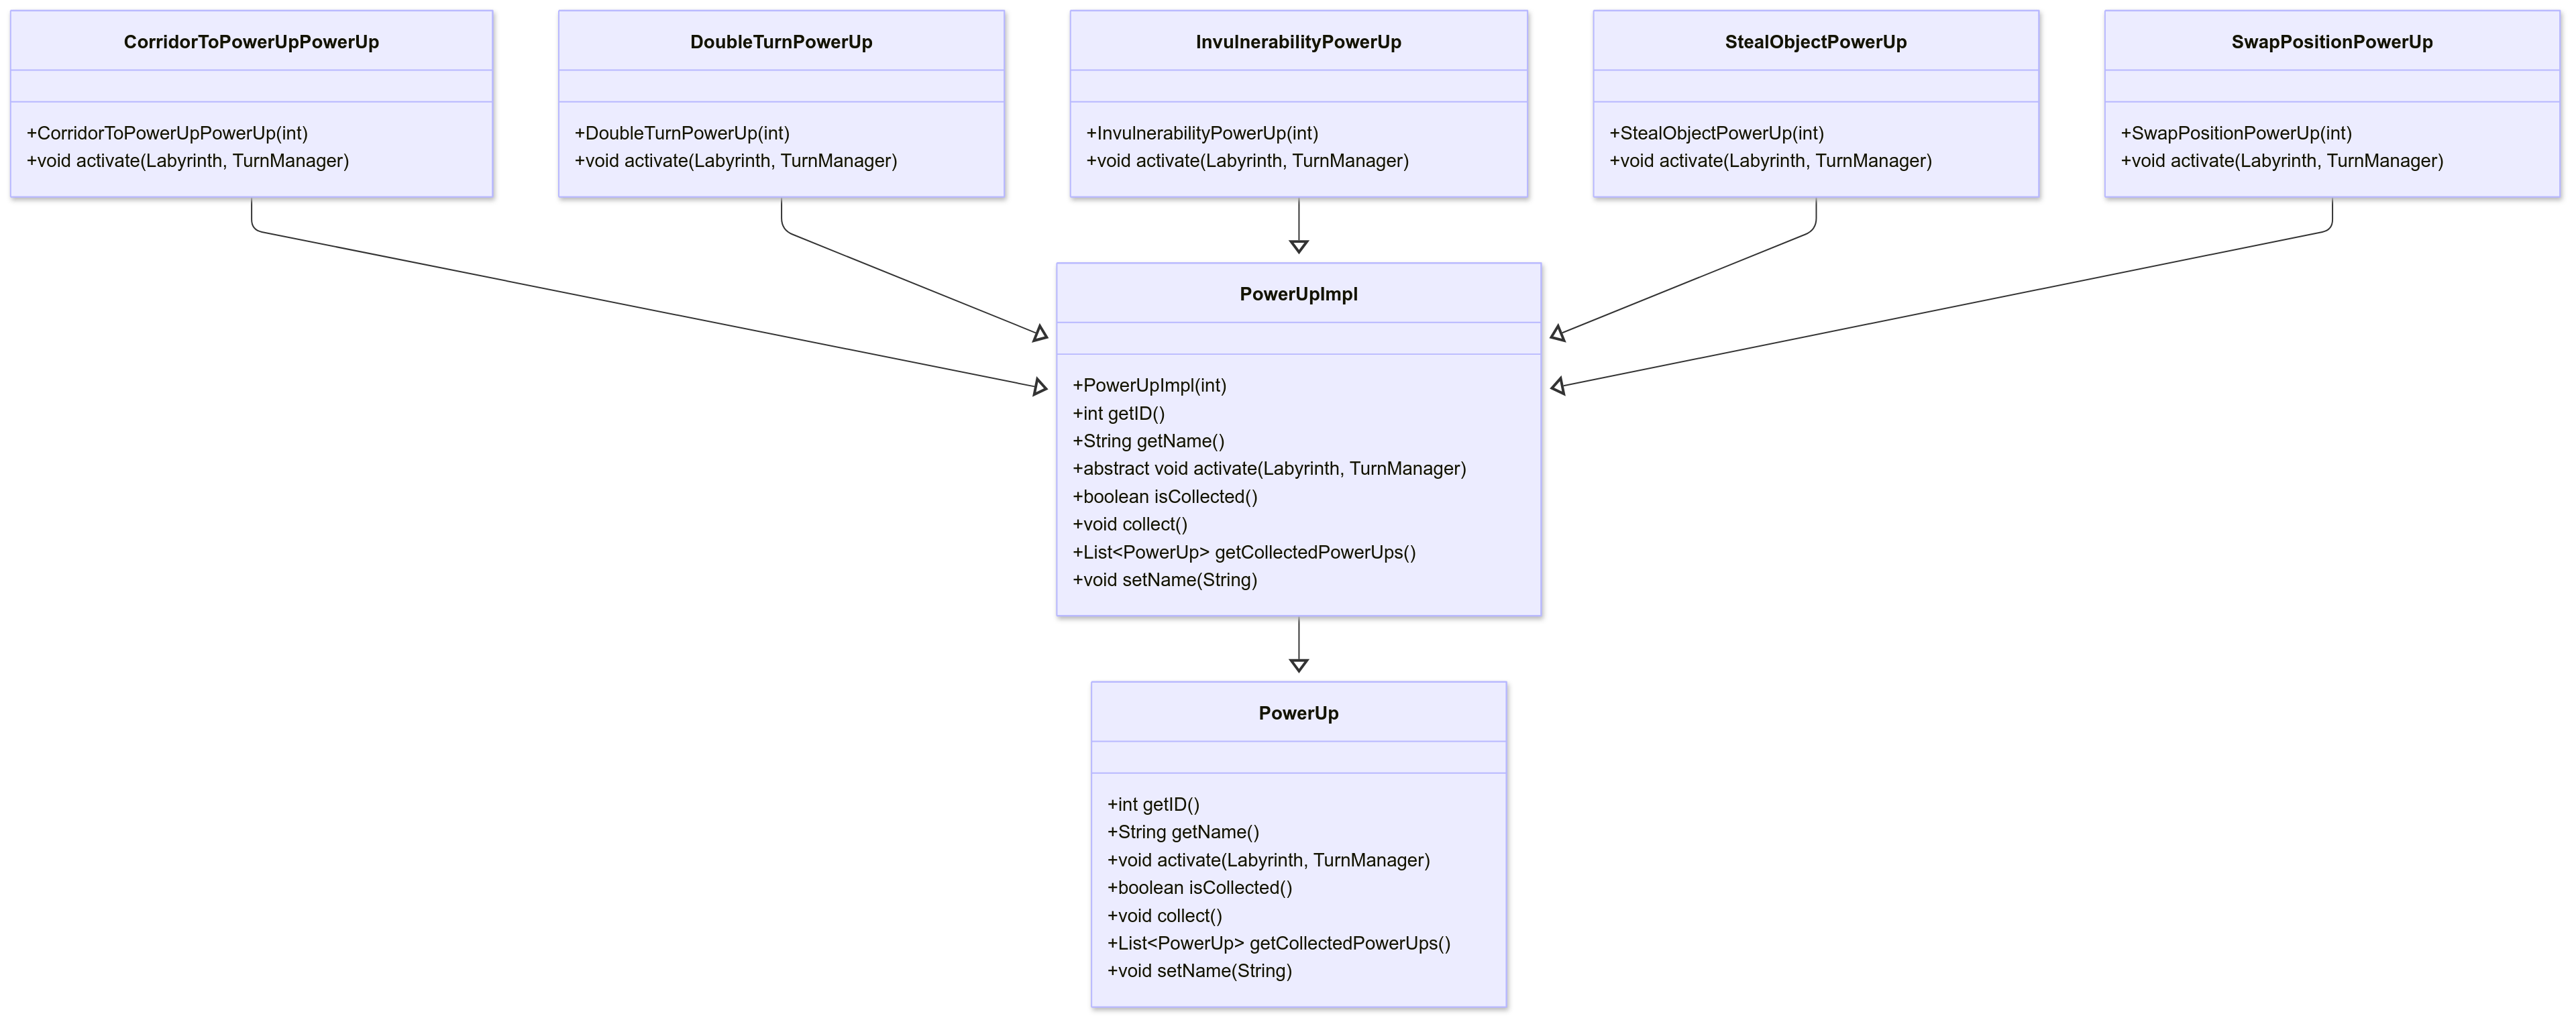
\includegraphics[width=14cm]{img/GestionePowerUp.png}
	\caption{Schema UML della gestione dei Power-Up}
	\label{img:Gestione PowerUp}
\end{figure}

\newpage
\subsubsection*{Gestione del Menu Principale e delle Impostazioni}

\paragraph{PROBLEMA}  
All'avvio dell'applicazione era necessario fornire all’utente un'interfaccia grafica iniziale per avviare una nuova partita, caricare una partita salvata, modificare le impostazioni o uscire dal gioco. Inoltre, non era presente un sistema per configurare i parametri della partita (numero di giocatori, presenza del nemico, numero di power-up, difficoltà del nemico).

\paragraph{SOLUZIONE}  
Per risolvere questo problema, ho implementato le componenti del \textit{Main Menu} e del relativo sistema di gestione delle impostazioni.
Nello specifico:
\begin{itemize}
    \item Ho creato l’interfaccia \texttt{MainMenuController} e la sua implementazione \texttt{MainMenuControllerImpl}, che gestisce tutte le interazioni provenienti dal menu principale: avvio di una nuova partita, caricamento dell’ultima partita salvata e apertura del menu delle impostazioni.
    \item Ho realizzato la classe \texttt{MainMenu}, una \texttt{JFrame} che rappresenta l'interfaccia grafica del menu principale. I bottoni presenti comunicano con il controller attraverso \texttt{listener} che attivano i metodi corrispondenti.
    \item Ho anche implementato l’interfaccia \texttt{SettingsController} e la sua implementazione \texttt{SettingsControllerImpl}, responsabili di comunicare al \texttt{SaveController} le impostazioni scelte dall’utente. Queste impostazioni vengono poi utilizzate per inizializzare correttamente la partita.
\end{itemize}
\begin{figure}[H]
	\centering{}
	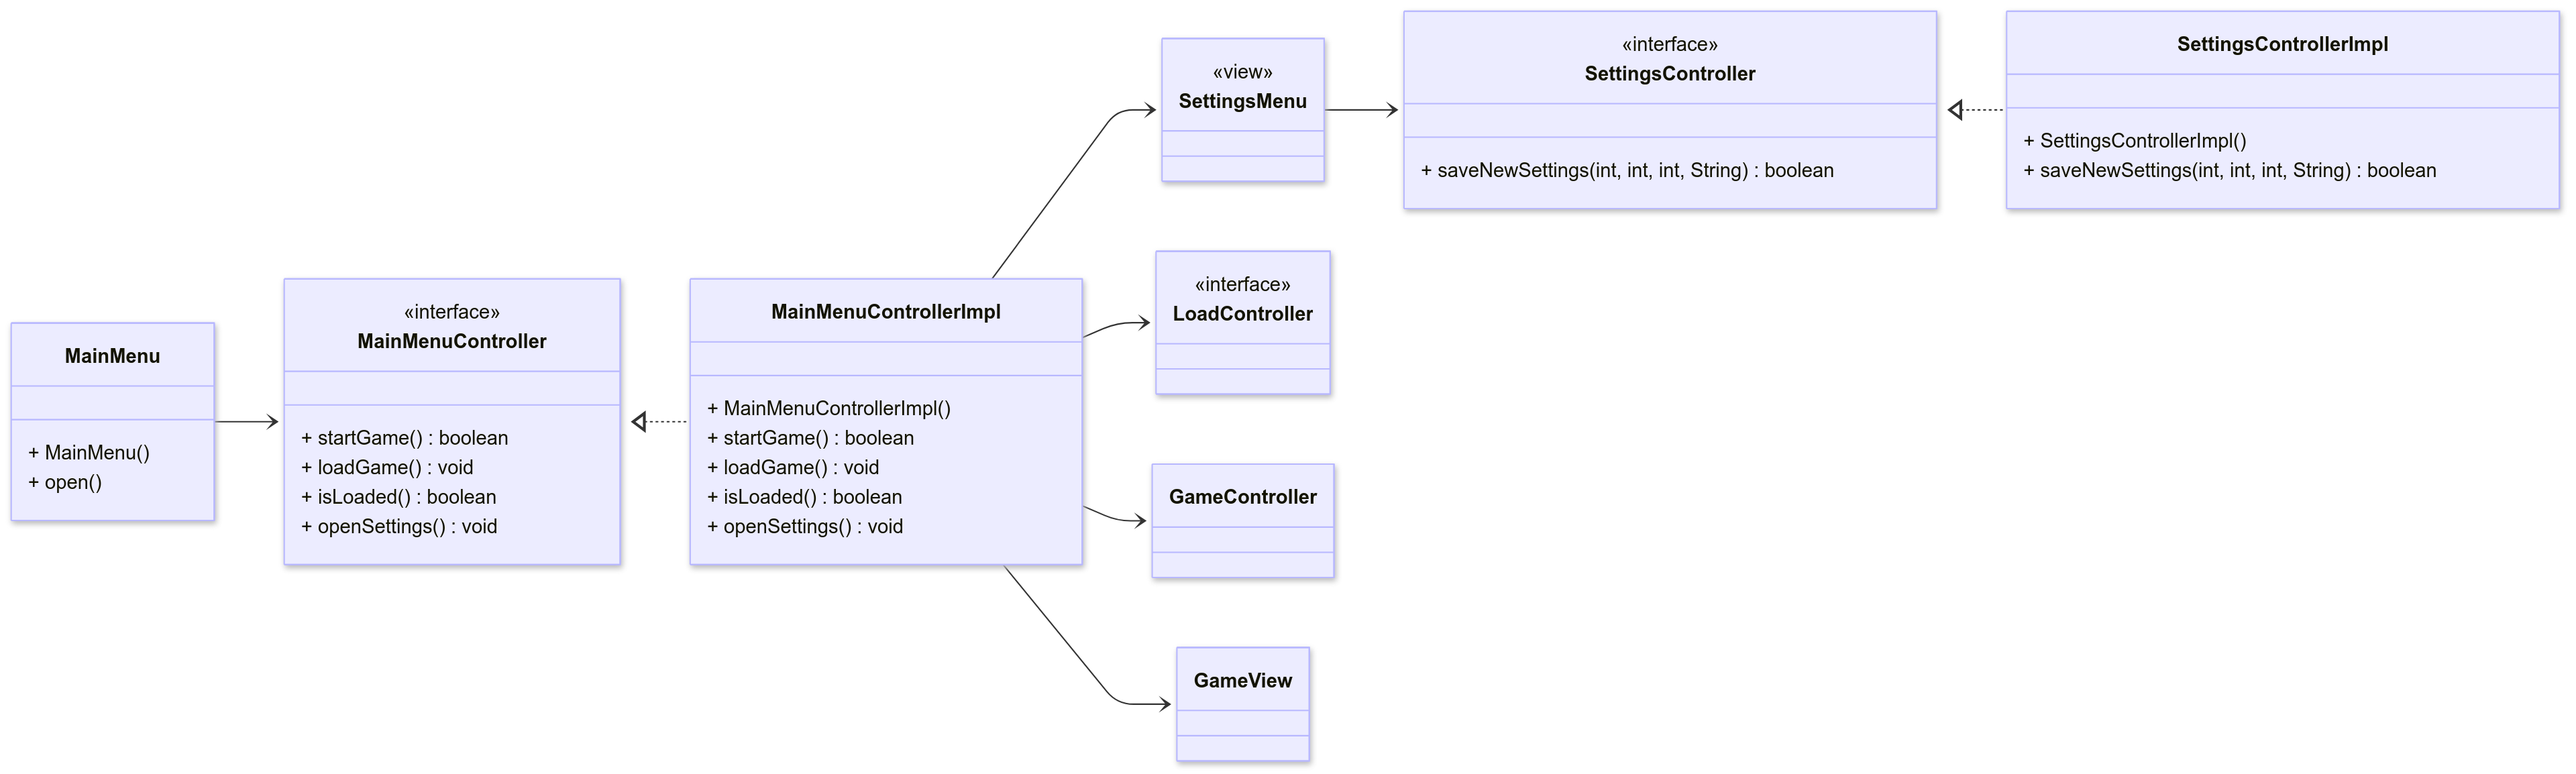
\includegraphics[width=14cm]{img/MainMenu.png}
	\caption{Schema UML della gestione del Main Menu e delle Impostazioni}
	\label{img:Gestione MainMenu}
\end{figure}


\chapter{Sviluppo}
\section{Testing automatizzato}

Per verificare il corretto funzionamento delle diverse parti del progetto, sono
 stati creati Test automatizzati usando JUnit.

\subsection{Enrico Ancarani}
\begin{itemize}
	\item \textbf{BlockTest}: verifica la corretta creazione delle tessere e il funzionamento della rotazione. I test accertano che, a seguito della rotazione, 
	l’orientamento della tessera cambi come previsto.
	\item \textbf{GenerateMazeTest}: verifica la correttezza della generazione iniziale della mappa di gioco. In particolare, si controlla che:
	\begin{itemize}
		\item tutte le tessere abbiano coordinate valide all’interno del labirinto.
		\item non vi siano duplicati (ovvero, che ogni tessera sia presente in una sola posizione).
		\item il blocco esterno venga generato correttamente.
		\item i blocchi iniziali dei giocatori siano posizionati correttamente.
	\end{itemize}
	\item \textbf{PositioningTest}: controlla che ogni elemento abbia una posizione nel labirinto e che i giocatori siano inizilizzati nelle giuste posizioni.
	Poi controlla che se effettuata una modifica alla posizione di un elemento essa non presenta errori e viene salvata correttamente.
	\item \textbf{ShiftsTest}: verifica il comportamento dello shift del labirinto. Dopo l’esecuzione dello spostamento, si controlla che 
	tutte le tessere siano state aggiornate nella posizione corretta e che il blocco esterno sia stato gestito coerentemente.
	\item \textbf{PlayerTest}: verifica il corretto comportamento del player nelle situazioni:
	\begin{itemize}
		\item raccolta di un obbietivo.
		\item utilizzo di un powerUp.
		\item movimento.
	\end{itemize}
\end{itemize}

\subsection{Stefano Baiano}
\begin{itemize}
	\item \textbf{DirectionCheckTest}: verifica che la classe DirectionCheck funzioni correttamente. Ogni Test controlla la singola 
	entrata laterale per i tre tipi di blocchi in tutte le quattro direzioni possibili
	\item \textbf{ActionCheckTest}: verifica se i controlli di movimento del giocatore e del nemico che vengono trattati dall'ActionPredicate
	funzionino senza intoppi. Prima testa il giocatore con delle situazioni in cui non è possibilitato a muoversi per vedere se il risultato 
	viene corretto, lo stesso test viene infine riproposto al nemico.
\end{itemize}

\newpage
\subsection{Andrea Monti}
\begin{itemize}
	\item \textbf{TurnManagerTest}: verifica che le azioni di turno dei giocatori si susseguano nell’ordine corretto, 
	ovvero prima il posizionamento del blocco e poi il movimento del giocatore. 
	Inoltre, controlla che il giocatore attivo rimanga lo stesso per l’intera durata del turno (due azioni consecutive) e 
	che, al termine di queste, il turno passi correttamente al giocatore successivo.
	\item \textbf{BuilderImplTest}: ha lo scopo di verificare che il costruttore inizializzi correttamente 
	tutti gli elementi del labirinto. In particolare, viene controllato che vengano generati due giocatori, che il nemico 
	sia presente e correttamente posizionato, che i PowerUp siano creati nella quantità prevista e che il labirinto venga 
	generato correttamente, restituendo un oggetto non nullo.
	\item \textbf{EnemyTest}: si occupa di verificare il comportamento del nemico in relazione alla difficoltà impostata. In modalità
	EASY, il nemico si muove solo di una posizione randomica; in modalità MEDIUM, cerca di avvicinarsi ai 
	giocatori muovendosi per un numero casuale di passi; mentre in modalità HARD, riesce a raggiungere il giocatore più vicino se è 
	presente una strada percorribile. Inoltre, viene controllato che, in caso di impatto con un giocatore, il nemico provochi 
	la perdita di un obiettivo raccolto da parte del giocatore colpito.
\end{itemize}

\newpage
\subsection{Simone Alocchi}
\begin{itemize}
	\item \textbf{DoubleTurnPowerUpTest}: 
	l'obbiettivo è verificare che il giocatore ottenga un secondo turno consecutivo dopo l’attivazione.  
	In questo test si assegna il power-up al giocatore attivo, lo si raccoglie e lo si attiva.  
	Si verifica che, dopo il normale passaggio di turno, il turno rimanga ancora al giocatore stesso, confermando l’effetto corretto.
	\item \textbf{SwapPositionPowerUpTest}: 
	l'obbiettivo è scambiare le posizioni dei due giocatori.  
	In questo test si salvano le coordinate iniziali dei due giocatori, poi si attiva il power-up.  
	Il test verifica che le coordinate dei due giocatori risultino invertite.
	\item \textbf{InvulnerabilityPowerUpTest}:
	l'obbiettivo è rendere temporaneamente invulnerabile il giocatore.  
	In questo test si attiva il power-up, si muove il giocatore nella posizione di un nemico e si verifica che, 
	nonostante l’incontro, il giocatore non subisca effetti negativi.
	\item \textbf{StealObjectPowerUpTest}: 
	l'obbiettivo è rubare un oggetto (power-up) a un altro giocatore.  
	In questo test il primo giocatore attiva il power-up mentre il secondo possiede un altro power-up.  
	Dopo l’attivazione, si verifica che il primo giocatore abbia entrambi gli oggetti.
	\item \textbf{CorridorToPowerUpPowerUpTest}: 
	l'obbiettivo è creare un corridoio diretto verso un power-up non raccolto.  
	Questa funzione è testata in più casi, ciascuno con diversa posizione del target.
	In ogni test, il giocatore e il target vengono posizionati in coordinate specifiche.  
	Dopo l’attivazione, il giocatore segue il corridoio generato e raccoglie il power-up target.  
	Il test si assicura che l’effetto sia correttamente applicato e che la strada generata sia percorribile e coerente con le regole del labirinto.
\end{itemize}

\section{Note di sviluppo}

\subsection{Enrico Ancarani}
\begin{itemize}
	\item \textbf{Utilizzo di Optional}: Utilizzato in vari punti, un esempio è: \url{https://github.com/EnricoAncaraniUnibo/OOP24-LabiOOPint/blob/bff4699198b12c8ac5b1b91a798ec85b5443a107/src/main/java/labioopint/model/maze/impl/MazeImpl.java#L46}
	\item \textbf{Utilizzo di Stream}: Utilizzato in vari punti, un esempio è: \url{https://github.com/EnricoAncaraniUnibo/OOP24-LabiOOPint/blob/bff4699198b12c8ac5b1b91a798ec85b5443a107/src/main/java/labioopint/model/maze/impl/LabyrinthImpl.java#L355}
	\item \textbf{Utilizzo di Lambda expressions}: Utilizzato nella classe LabyrinthImpl: \url{https://github.com/EnricoAncaraniUnibo/OOP24-LabiOOPint/blob/bff4699198b12c8ac5b1b91a798ec85b5443a107/src/main/java/labioopint/model/maze/impl/LabyrinthImpl.java#L386}
\end{itemize}

\subsection{Stefano Baiano}
\begin{itemize}
	\item \textbf{Utilizzo di FileOutputStream}: Utilizzo nella classe SaveControllerImpl: \url{https://github.com/EnricoAncaraniUnibo/OOP24-LabiOOPint/blob/bff4699198b12c8ac5b1b91a798ec85b5443a107/src/main/java/labioopint/controller/impl/SaveControllerImpl.java#L49}
	\item \textbf{Utilizzo di FileInputStream}: Utilizzo nella classe LoadControllerImpl: \url{https://github.com/EnricoAncaraniUnibo/OOP24-LabiOOPint/blob/bff4699198b12c8ac5b1b91a798ec85b5443a107/src/main/java/labioopint/controller/impl/LoadControllerImpl.java#L80}
\end{itemize}

\subsection{Andrea Monti}
\begin{itemize}
	\item \textbf{Utilizzo di Optional}: Utilizzato in vari punti, un esempio è: \url{https://github.com/EnricoAncaraniUnibo/OOP24-LabiOOPint/blob/ecece579eb253c22447203ab5b4b3d95ae79cd1d/src/main/java/labioopint/model/enemy/impl/ais/ChaseAI.java#L66}
	\item \textbf{Utilizzo di Stream}: Utilizzato in vari punti, un esempio è: \url{https://github.com/EnricoAncaraniUnibo/OOP24-LabiOOPint/blob/ecece579eb253c22447203ab5b4b3d95ae79cd1d/src/main/java/labioopint/model/enemy/impl/ais/ChaseAI.java#L68-L70}
\end{itemize}

\subsection{Simone Alocchi}
\begin{itemize}
	\item \textbf{Utilizzo di lambda expressions, stream e Optional}: \url{https://github.com/EnricoAncaraniUnibo/OOP24-LabiOOPint/blob/465bc960d57def0ff2b8337927578b86720b918b/src/main/java/labioopint/model/powerup/impl/StealObjectPowerUp.java#L33}
\end{itemize}

\chapter{Commenti finali}

In quest'ultimo capitolo si tirano le somme del lavoro svolto e si delineano eventuali sviluppi
futuri.

\textit{Nessuna delle informazioni incluse in questo capitolo verrà utilizzata per formulare la valutazione finale}, a meno che non sia assente o manchino delle sezioni obbligatorie.
%
Al fine di evitare pregiudizi involontari, l'intero capitolo verrà letto dai docenti solo dopo aver formulato la valutazione.

\section{Autovalutazione e lavori futuri}

\subsection{Enrico Ancarani}
Questa non rappresentava la mia prima esperienza di lavoro in team per lo sviluppo di un progetto software complesso. 
Per questo motivo, ritengo che la mia presenza all'interno del gruppo sia stata un supporto utile anche per gli altri membri, sia dal punto di vista tecnico che organizzativo.
Il mio ruolo si è concentrato principalmente sulla modellazione della mappa di gioco, sulla gestione delle coordinate e degli elementi associati alla mappa, 
sull’aggiornamento grafico delle immagini e sulla gestione della logica relativa ai giocatori. Ho partecipato attivamente a ogni fase del progetto, mettendo impegno 
costante durante gli incontri e lavorando in modo continuativo tra una sessione e l’altra.
Tra i miei punti di forza riconosco la determinazione nel portare a termine le attività assegnate senza rimandare, la capacità di spiegare con chiarezza aspetti 
implementativi complessi agli altri membri del gruppo, e l'iniziativa nel proporre soluzioni rapide ed efficaci ai problemi riscontrati durante la scrittura del codice. 
Inoltre, ho cercato di mantenere alta la motivazione del team nei momenti di difficoltà.
D’altra parte, tra i miei punti di debolezza evidenzio una certa testardaggine nel difendere le mie proposte e la tendenza ad assumere un ruolo di leadership anche 
quando non esplicitamente richiesto, specialmente durante la fase di progettazione dell’architettura.
Le principali difficoltà riscontrate hanno riguardato l’utilizzo efficace di GitHub per il lavoro collaborativo e l’applicazione corretta e coerente del pattern 
architetturale MVC, soprattutto nelle prime fasi di sviluppo.
In conclusione, considero il mio contributo positivo e sono soddisfatto dell’impegno personale e del risultato ottenuto. 
Se in futuro si decidesse di proseguire con lo sviluppo del progetto, si potrebbe arricchire il gioco introducendo nuovi obiettivi, 
power-up, scenari alternativi con tessere speciali o strutture della mappa più articolate, al fine di aumentare la varietà e la profondità dell’esperienza di gioco.

\subsection{Stefano Baiano}
Riconosco che il mio ruolo all'interno del progetto è stato non costante data la situazione di lavoro accostato allo studio, motivo per il quale non sono riuscito 
ad essere sempre reperibile e presente durante tutti gli incontri. Sebbene questo mio punto a sfavore ritengo che la mia presenza durante gli incontri sia stata di 
aiuto per la costruzione dell'architettura del progetto e per mantenere un po' di leggerezza durante la progettazione per rimanere produttivi anche in sessioni più lunghe. 
La mia parte di lavoro è stata svolta principalmente da solo, vista la poca presenza, e quindi mi sono occupato di gestire il cuore di scambi di informazioni tra le varie classi 
create dai miei compagni, quali TurnManager e Labyrinth, una volta finita la loro parte. Inoltre mi sono occupato di gestire una serie di controlli per la gesione delle 
azioni che vengono effettuate da un utente. Sicuramente la mia parte è stata utile e tranquilla, dimostro una buona resa in poco tempo sebbene ho la tendenza a riempire 
la mia agenda di cose nuove da fare. Questa esperienza non rappresenta il mio primo lavoro in gruppo, sia per il mio lavoro attuale che per altri progetti tenuti in sede scolastica 
ho avuto la possibilità di fare grossi progetti che tutt'ora sono in uso e funzionanti.

\subsection{Andrea Monti}
Il mio ruolo principale è stato quello di progettare e implementare la logica dei turni e del nemico (compresa 
l’intelligenza di inseguimento), assicurandomi che il comportamento fosse coerente, sfidante e ben integrato con il 
resto del sistema. Mi sono occupato anche dell’implementazione del sistema di gestione dei turni, che coordina le azioni 
tra giocatori, nemici e power-up, e della generazione degli oggetti della partita, tra cui la creazione del labirinto, dei 
giocatori, dei power-up e del nemico, con comportamenti variabili in base alla difficoltà selezionata.
Sono molto soddisfatto del lavoro svolto, sia individualmente che in gruppo. Abbiamo completato con successo tutte le 
funzionalità obbligatorie e alcune opzionali, mantenendo sempre un forte spirito di collaborazione.
In futuro mi piacerebbe tornare su questo progetto per estendere ulteriormente il comportamento del nemico, 
magari introducendo un nemico ancora più potente o nuove modalità di gioco. Grazie alla struttura modulare e all’attenzione 
riposta nella manutenibilità del codice, sono certo che queste e altre modifiche saranno facilmente realizzabili.

\subsection{Simone Alocchi}
Il mio compito nel progetto era principalmente quello di gestire le funzionalità dei power-up, nonché degli obiettivi di gioco, e della creazione del menu iniziale.  
Mi posso ritenere abbastanza soddisfatto del mio lavoro, in quanto sono riuscito a completare tutti i power-up che mi ero prefissato di fare, incluso \texttt{CorridorToPowerUpPowerUp}, 
che ritengo discretamente complesso, oltre a sviluppare un menu con grafica e funzionalità in linea con il resto del progetto.  
Sono riuscito a mantenere coerenza con i principi MVC e DRY, e la progettazione modulare adottata renderà semplice l’aggiunta di nuove funzionalità in futuro.  
Il lavoro di gruppo è andato abbastanza bene e siamo riusciti a rispettare le date di scadenza senza particolari difficoltà.
\\
\\
\appendix
\chapter{Guida utente}

All'apertura del sofware il programma presenta un menù per garantire al/agli utente/i di poter scegliere la modalità richiesta. 
Nel caso non si voglia iniziare una partita con impostazioni standard è importante andare all'interno dell'opzione "Settings" salvando alla fine dei cambiamenti effettuati.
Appena confermate le impostazioni si può premere il tasto "Start Game" per iniziare la partita con le caratteristiche scelte.

\subsection*{Come giocare}

Ogni giocatore ha a disposizione due azioni che si svolgono obbligatoriamente con uno specifico ordine.

\begin{itemize}
 \item Posizionamento del blocco. Si può girare il blocco tramite l'uso delle frecce laterali(rosso nell'immagine), una volta soddisfatti si può piazzare il blocco dove si preferisce cliccando nelle parti esterne del labirinto, escluso gli angoli(blu nell'immagine).
 \begin{figure}[H]
	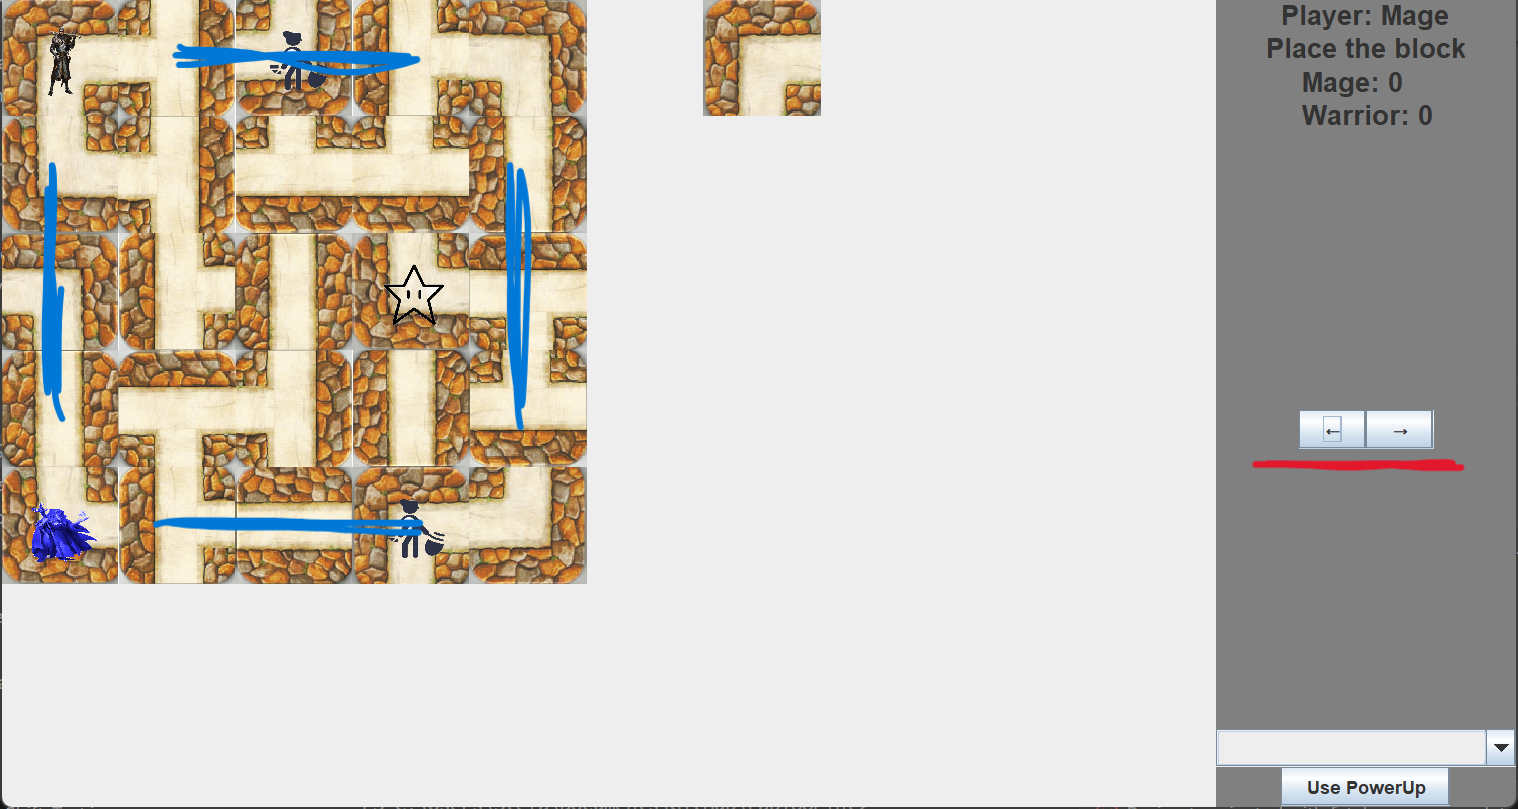
\includegraphics[width=\textwidth]{img/EsempioDiPrimoTurno.png}
	\caption{Immagine di una partita in att}
	\label{img:Esempio di primo turno}
 \end{figure}
 \item Movimento del giocatore. Il giocatore potrà muoversi liberamente all'interno del labirinto, senza passare le pareti, usando le frecce laterali. Per terminare il suo turno e passarlo a quello successivo dovrà premere in basso a destra il tasto "End Turn".
\end{itemize}

\subsection*{Nemico}

All'interno del gioco ci sarà un nemico che cercherà di prendervi alla fine del vostro turno. Se si viene presi vi verrà sottriatto un powerUp e rimesso nel campo di gioco.

\subsection*{PowerUp}

All'interno del gioco si possono collezionare powerUp passandoci sopra col proprio personaggio. Questi powerUp si possono utilizzare durante il 
proprio turno tramite il menù a tendina in passo a destra, una volta selezionato il powerUp desiderato bisogna premere il tasto "Usa powerUp" subito sotto

\subsection*{Obiettivo}

Per poter vincere bisogna avere più powerUp degli altri quando l'ultimo powerUp del labirinto è stato preso.

\chapter{Esercitazioni di laboratorio}

\subsection{andrea.monti24@studio.unibo.it}

\begin{itemize}
 \item Laboratorio 06: \url{https://virtuale.unibo.it/mod/forum/discuss.php?d=176282#p244949}
 \item Laboratorio 07: \url{https://virtuale.unibo.it/mod/forum/discuss.php?d=177162#p246019}
 \item Laboratorio 08: \url{https://virtuale.unibo.it/mod/forum/discuss.php?d=178723#p247248}
 \item Laboratorio 09: \url{https://virtuale.unibo.it/mod/forum/discuss.php?d=179154#p248230}
 \item Laboratorio 10: \url{https://virtuale.unibo.it/mod/forum/discuss.php?d=180101#p249109}
 \item Laboratorio 11: \url{https://virtuale.unibo.it/mod/forum/discuss.php?d=181206#p250502}
\end{itemize}

\subsection{simone.alocchi@studio.unibo.it}

\begin{itemize}
 \item Laboratorio 09: \url{https://virtuale.unibo.it/mod/forum/discuss.php?d=179154#p248408}
 \item Laboratorio 10: \url{https://virtuale.unibo.it/mod/forum/discuss.php?d=180101#p249975}
\end{itemize}

\end{document}
